\chapter{Softwaredesign}

\section{Dataprotokol (BS)}\label{header:dataprotokol}
%% SW design: Dataprotokol

\subsubsection{Aktiver, Deaktiver og Verificer}

Aktiver og Deaktiver handler ikke på enhedsnummeret.

Ved verificering af en Enhed sendes et enhedsnummer til Enheden, som der verificeres på i forhold til Enhedens enhedsnummer.

\begin{table}[h]
	\caption{Data-formatering for verificering}
	\centering
	\begin{tabular}{|l|c|}
		\hline 
		\textbf{Byte} & \textbf{Enhedsnummer} \\ 
		\hline 
		\textbf{Indhold} & ''\verb+NN+''\\ 
		\hline 
	\end{tabular} 
	\label{table:SWProtokol-verificer}
\end{table}

\subsubsection{Send parametre}

Ved parameter indstilling skal der sendes følgende parametre til Enheden.

\begin{enumerate}
	\item Enhedsnummer (1-18)
	\item Øvre temperaturgrænse
	\item Nedre fugtighedsgrænse
\end{enumerate}

Parametrene skal sendes i ovenstående rækkefølge og resulterer altså i en kommando som vist i tabel \ref{table:SWProtokol-para}. Temperaturgrænsen er begrænset til 3 heltal og én decimal. Fugtighedsgrænsen er begrænset til 3 heltal.

\begin{table}[h]
	\caption{Data-formatering for parametre}
	\centering
	\begin{tabular}{|l|c|c|c|}
		\hline 
		\textbf{Byte} & \textbf{Enhedsnummer} & \textbf{Temperatur} & \textbf{Fugtighed} \\ 
		\hline 
		\textbf{Indhold} & ''\verb+NN+'' & ''\verb+TTT.T+'' & ''\verb+FFF+''  \\ 
		\hline 
	\end{tabular} 
	\label{table:SWProtokol-para}
\end{table}

\subsubsection{Log}

Når data flyttes mellem Master og Enhed, ifm. logning, anvendes følgende dataprotokol i mellem \textit{Application}-lagene.

Den data som skal flyttes er følgende:

\begin{enumerate}
	\item Temperatur
	\item Fugtighed
	\item Bevægelsesregistrering
	\item Påbegyndt vanding
\end{enumerate}

Systemet ved ikke på forhånd hvor meget data der skal flyttes. Derfor deles det op i tre typer. Data fra sensorene, besked om bevægelse og fejlregistreringer.
Fælles for de tre er at tidsstemplet altid sendes med.

Fra standardbiblioteket for \verb'C++' vælges datatypen \verb+vector+ som container. Dette er en dynamisk array-struktur som automatisk udvides og mindskes efter behov.
Ved at anvende \verb+vector+en med \verb+string+ som undertype er det nemt at identificerer indholdene og formaterer dem som nødvendigt. På Enheden som implementeres på en PSoC er standardbiblioteket til \verb-C++- ikke tilrådighed. Derfor implementeres bufferen på denne som et almindeligt statisk allokeret char-array. Formateringen vist her under gælder for begge platforme.

Som nævnt er der flere muligheder for ''datapakker''. I tabellerne \ref{table:SWDataprotokol-sensor}, \ref{table:SWDataprotokol-bevaegelse} og \ref{table:SWDataprotokol-error} er deres opbygninger vist.

Første streng der læses afgør hvor mange af de efterfølgende strenge som høre her til. Hvis det første der modtages er ''\verb+D+'', betyder det at der kommer information fra sensorene og der skal læses fire efterfølgende strenge.
Hvis der modtages et ''\verb+E+'' er der en fejl og én streng med fejlkoden fra enheden læses.

\begin{table}[h]
	\caption{Dataformatering ifm. sensordata}
	\centering
	\begin{tabular}{|c|c|c|c|c|}
		\hline 
		\textbf{Type} & \textbf{Temperatur} & \textbf{Fugtighed} & \textbf{Vanding} & \textbf{Bevægelse}\\ 
		\hline 
		''\verb+D+'' & ''\verb+TTT.T+'' & ''\verb+FFF+'' & ''\verb+0+'' / ''\verb+1+'' & ''\verb+0+'' / ''\verb+1+'' \\ 
		\hline 
	\end{tabular} 
	\label{table:SWDataprotokol-sensor}
\end{table}

\begin{table}[h]
	\caption{Dataformatering ifm. fejl}
	\centering
	\begin{tabular}{|c|c|}
		\hline 
		\textbf{Type} & \textbf{Fejlkode} \\ 
		\hline 
		''\verb+E+'' & ''\verb+XXX+'' \\ 
		\hline 
	\end{tabular} 
	\label{table:SWDataprotokol-error}
\end{table}

Et eksempel på strukturen af en datahentning er vist i tabel \ref{table:SWDataprotokol-eksempel}. Her kan man se, at der siden sidste udlæsning har været hentet sensordata med værdierne 14.5 grader og 20\% fugtighed, der har ikke været tændt for sprinkleren men der har været bevægelse på hullet, \verb+D014.502001+ og der har også været en fejl 13, \verb+E013+.

\begin{table}[h]
	\caption{Dataformatering ifm. log-information}
	\centering
	\begin{tabular}{|c|c|}
		\hline
		\verb+vector<string>[0]+ & \verb+[1]+ \\
		\hline 
		''\verb+D014.502001+'' & ''\verb+E013+'' \\ 
		\hline 
	\end{tabular} 
	\label{table:SWDataprotokol-eksempel}
\end{table}

\section{Applikationsmodeller (JC BS)}
Selve designet af softwaren bygger på de følgende applikationsmodeller. Her laves der sekvens- og klassediagrammer over hver del af systemet samt klassebeskrivelser hvor funktionen for de enkelte metoder beskrives.

%% SW design: Applikationsmodeller

Selve designet af softwaren bygger på de følgende applikationsmodeller. Her laves der sekvens- og klassediagrammer over hver del af systemet samt klassebeskrivelser hvor funktionen for de enkelte metoder beskrives.

\subsection{Master}
Applikationsmodeller for Master.

\begin{figure}[htbp] \centering
{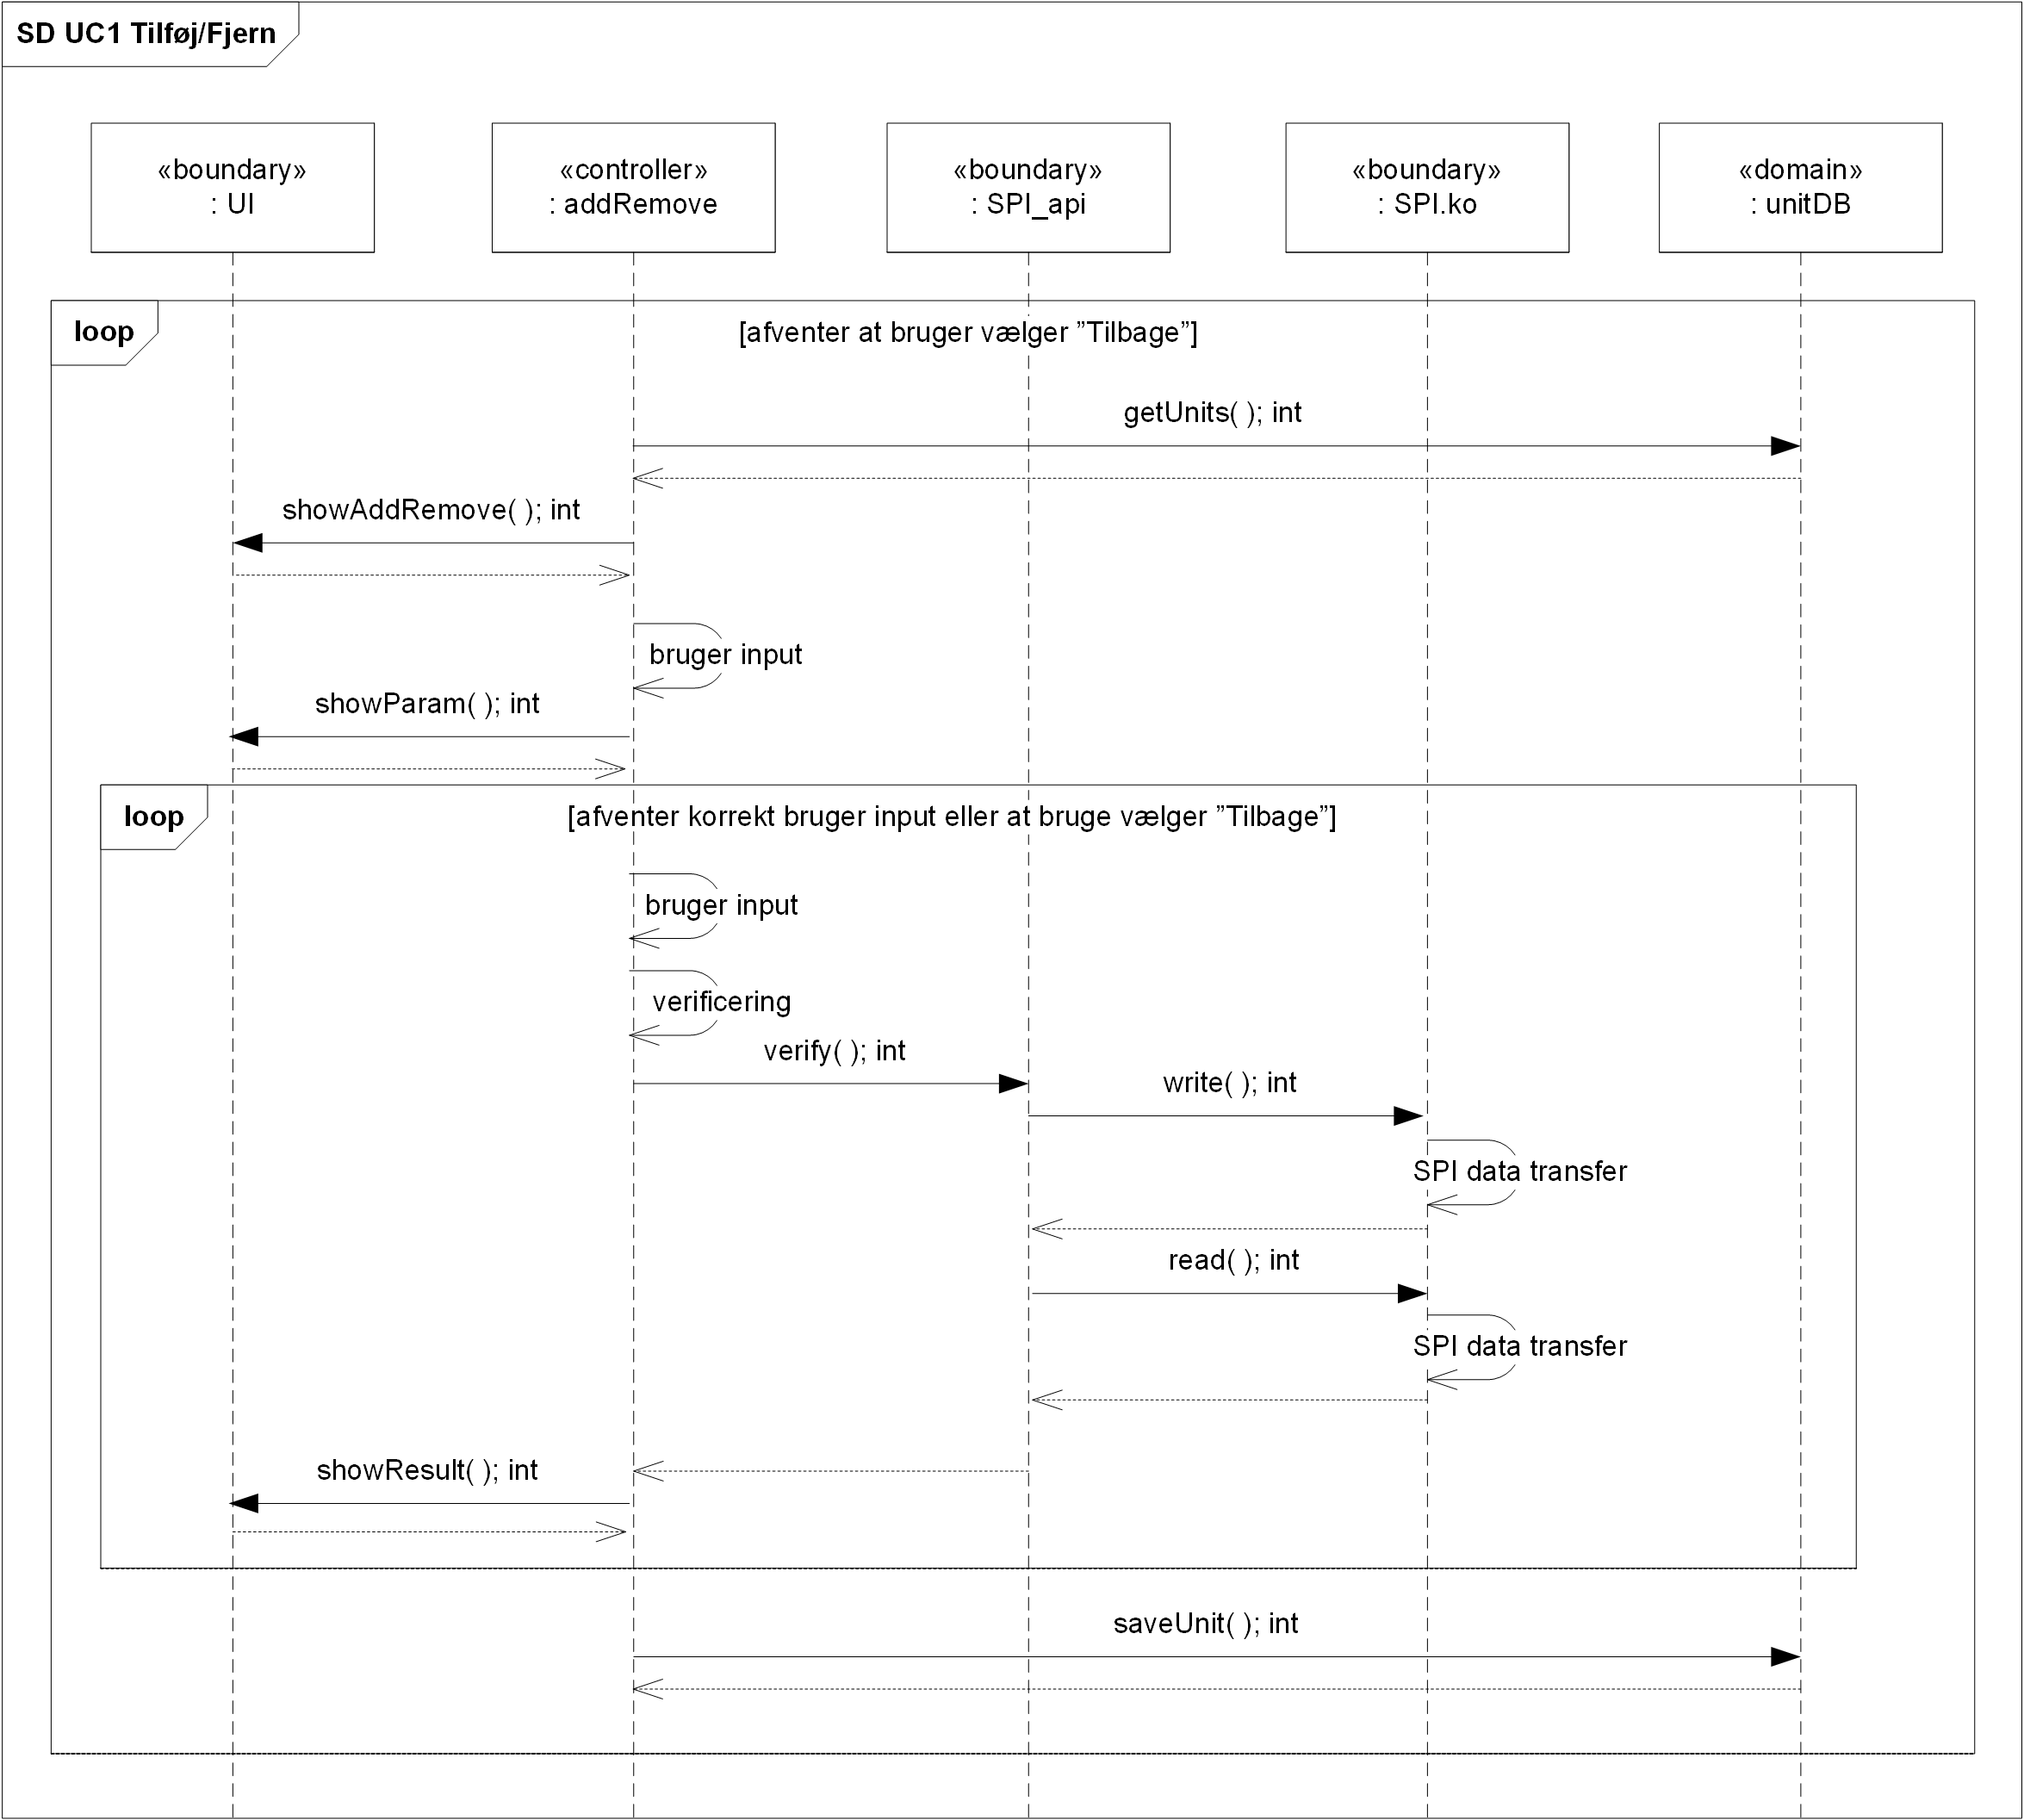
\includegraphics[scale=0.8]{filer/design/a_uc1}}
\caption{Sekvensdiagram UC1}
\label{fig:Sekvensdiagram UC1}
\end{figure} 

\begin{figure}[htbp] \centering
{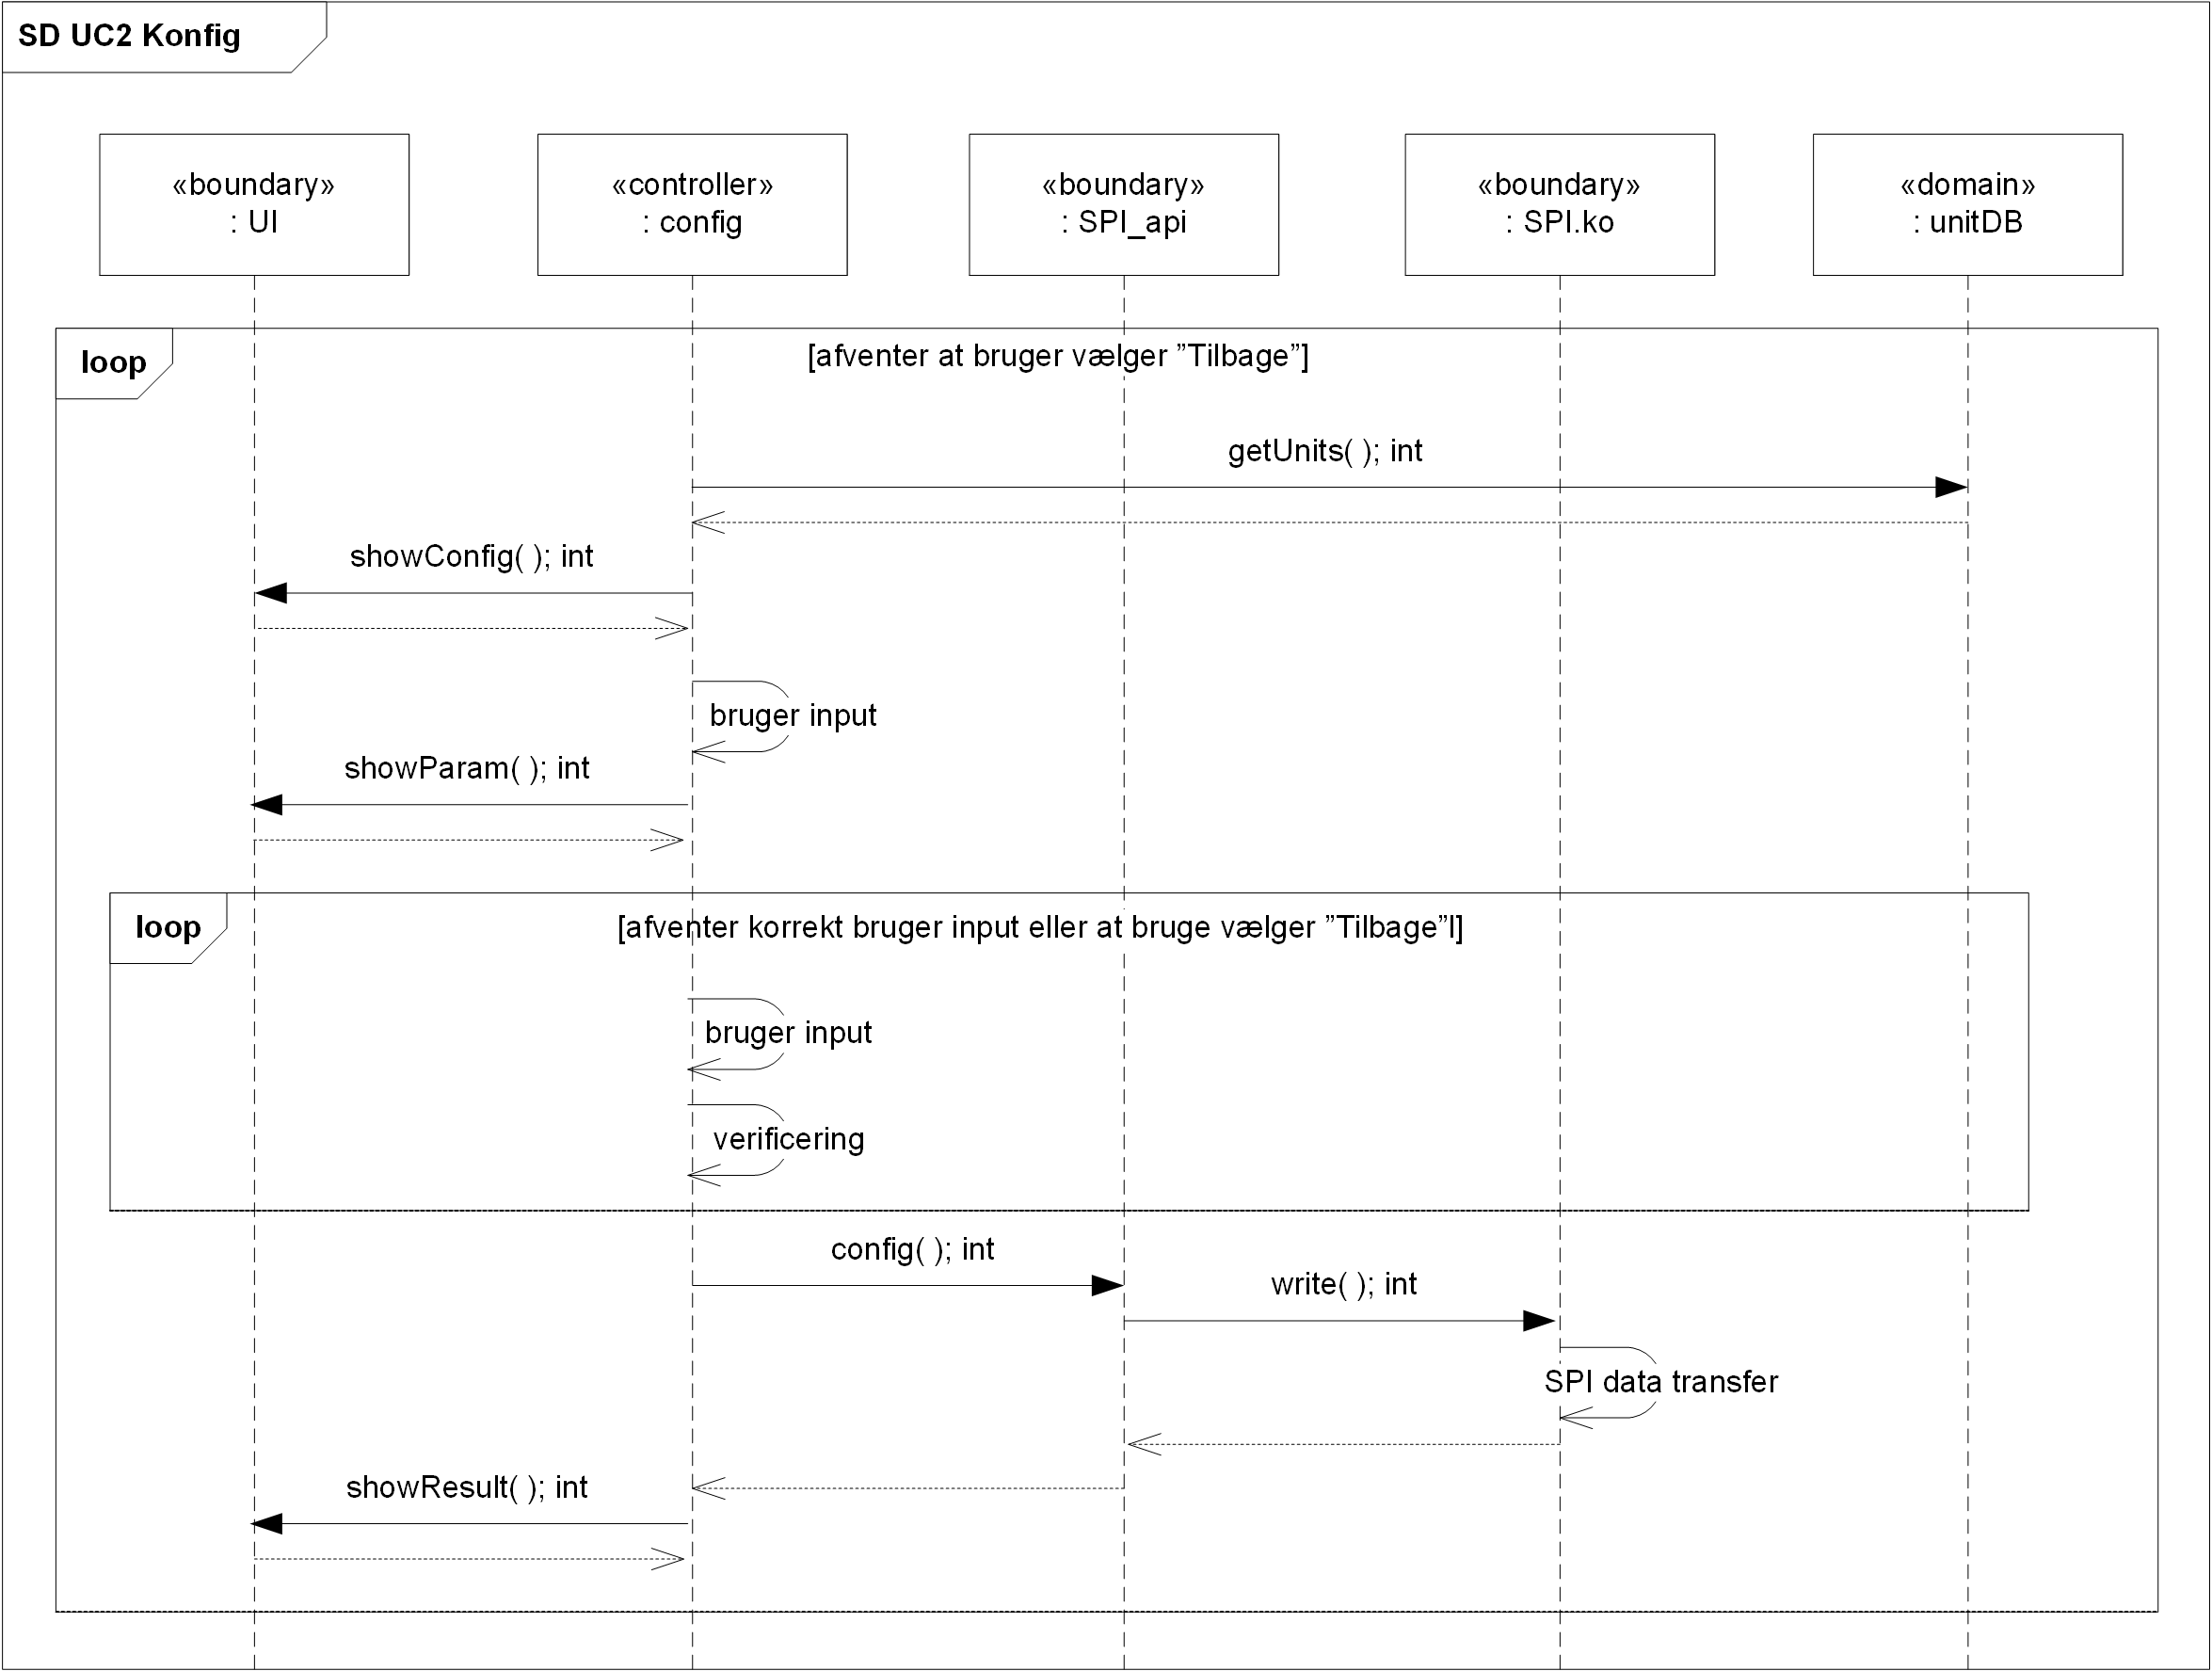
\includegraphics[scale=0.8]{filer/design/a_uc2}}
\caption{Sekvensdiagram UC2}
\label{fig:Sekvensdiagram UC2}
\end{figure} 

\begin{figure}[htbp] \centering
{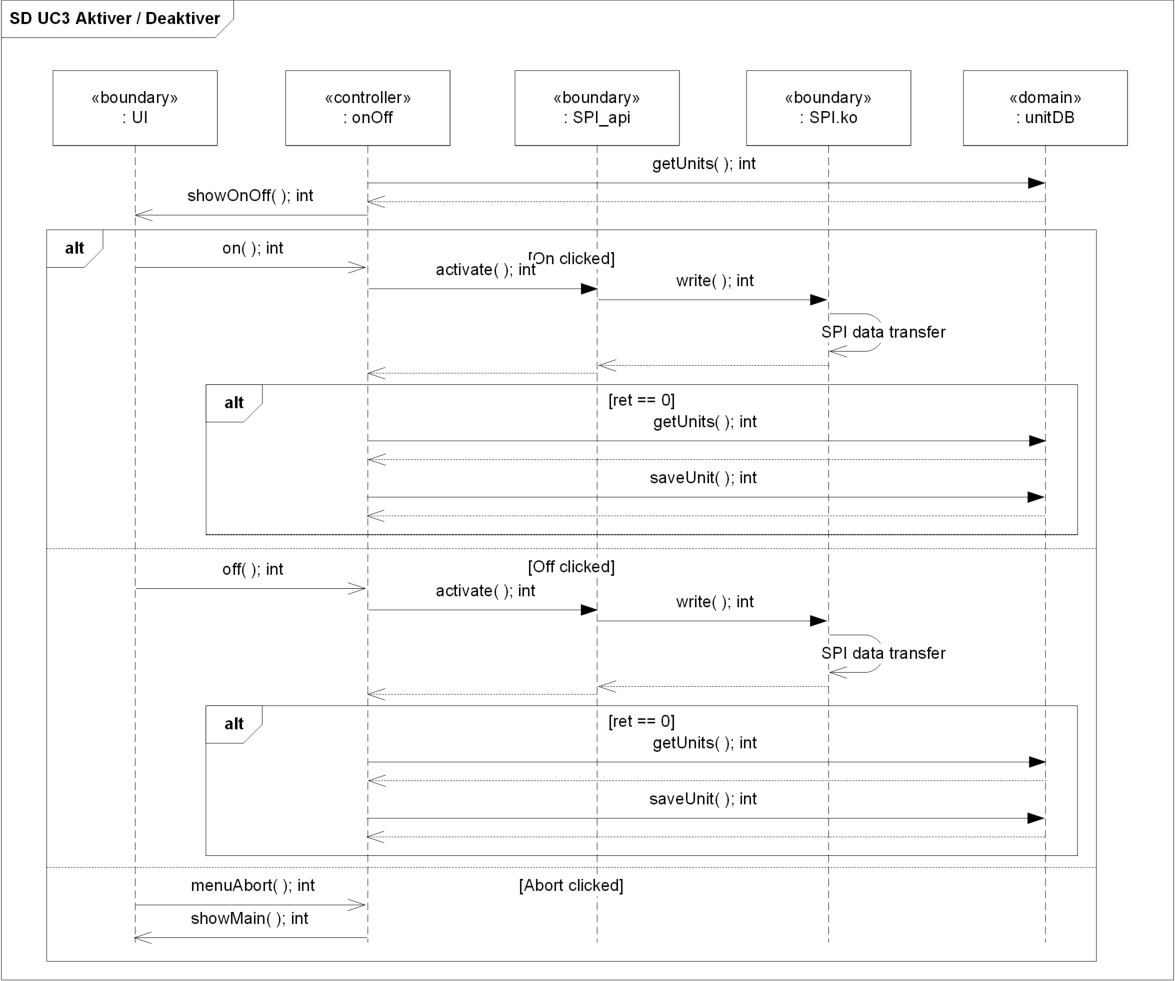
\includegraphics[scale=0.8]{filer/design/a_uc3}}
\caption{Sekvensdiagram UC3}
\label{fig:Sekvensdiagram UC3}
\end{figure} 

\begin{figure}[htbp] \centering
{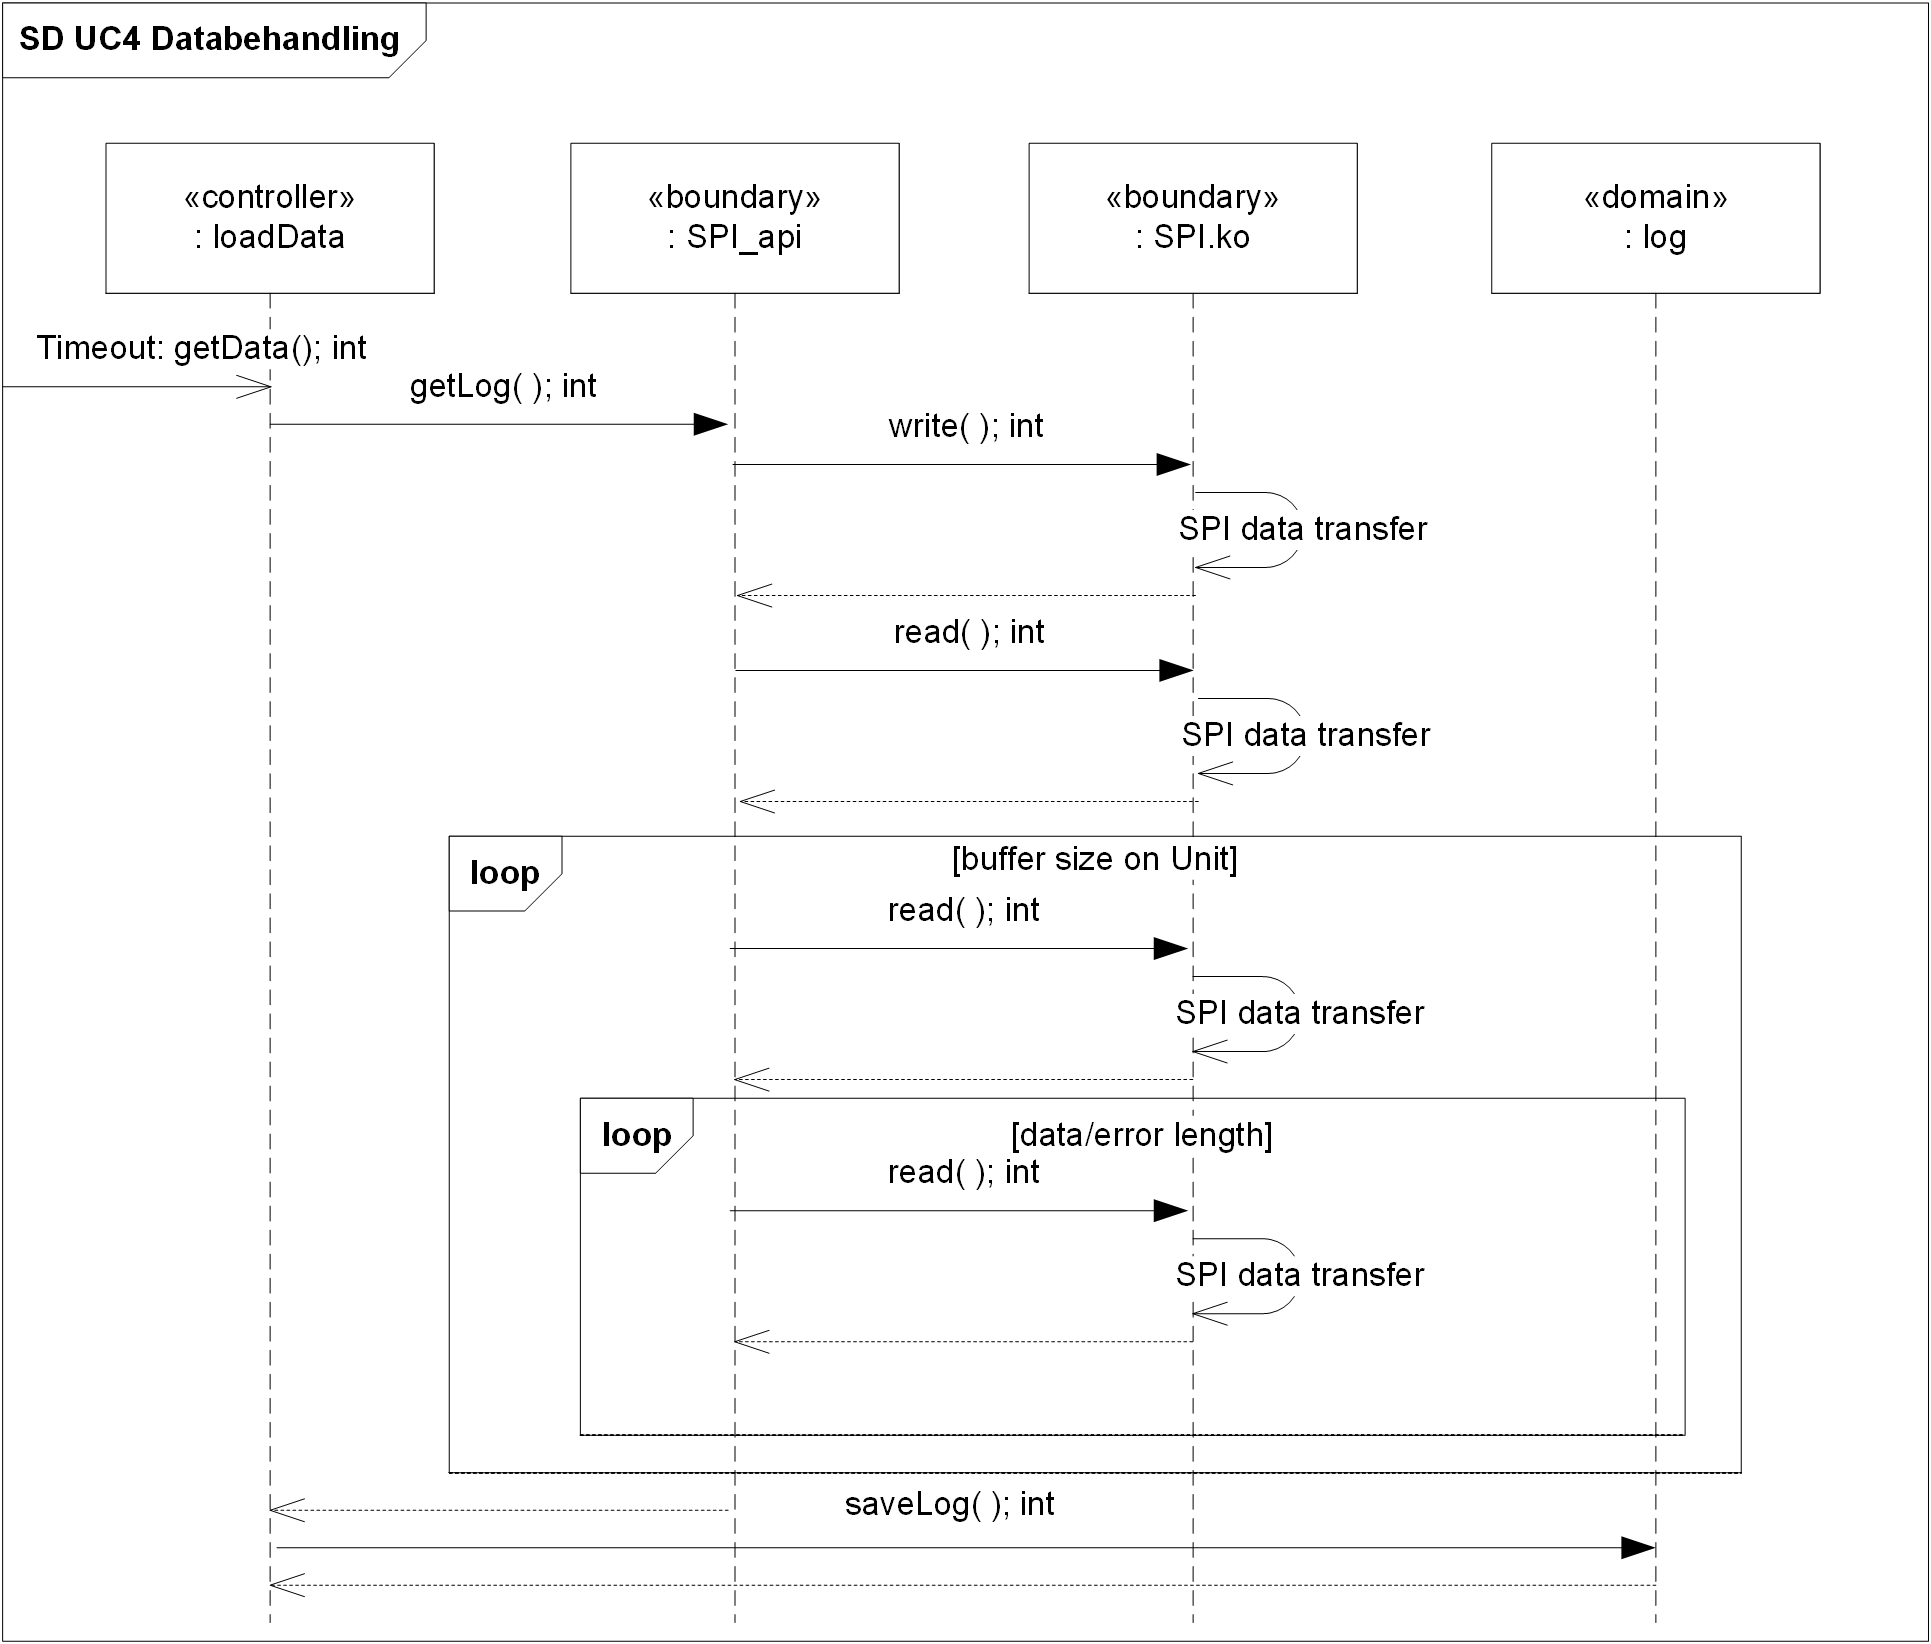
\includegraphics[scale=0.8]{filer/design/a_uc4}}
\caption{Sekvensdiagram UC4}
\label{fig:Sekvensdiagram UC4}
\end{figure} 

\begin{figure}[htbp] \centering
{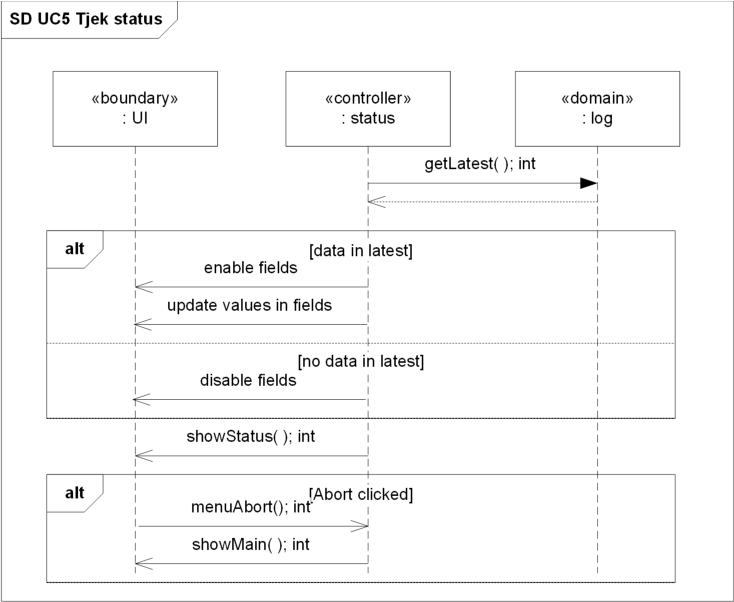
\includegraphics[scale=1]{filer/design/a_uc5}}
\caption{Sekvensdiagram UC5}
\label{fig:Sekvensdiagram UC5}
\end{figure} 

\begin{figure}[htbp] \centering
{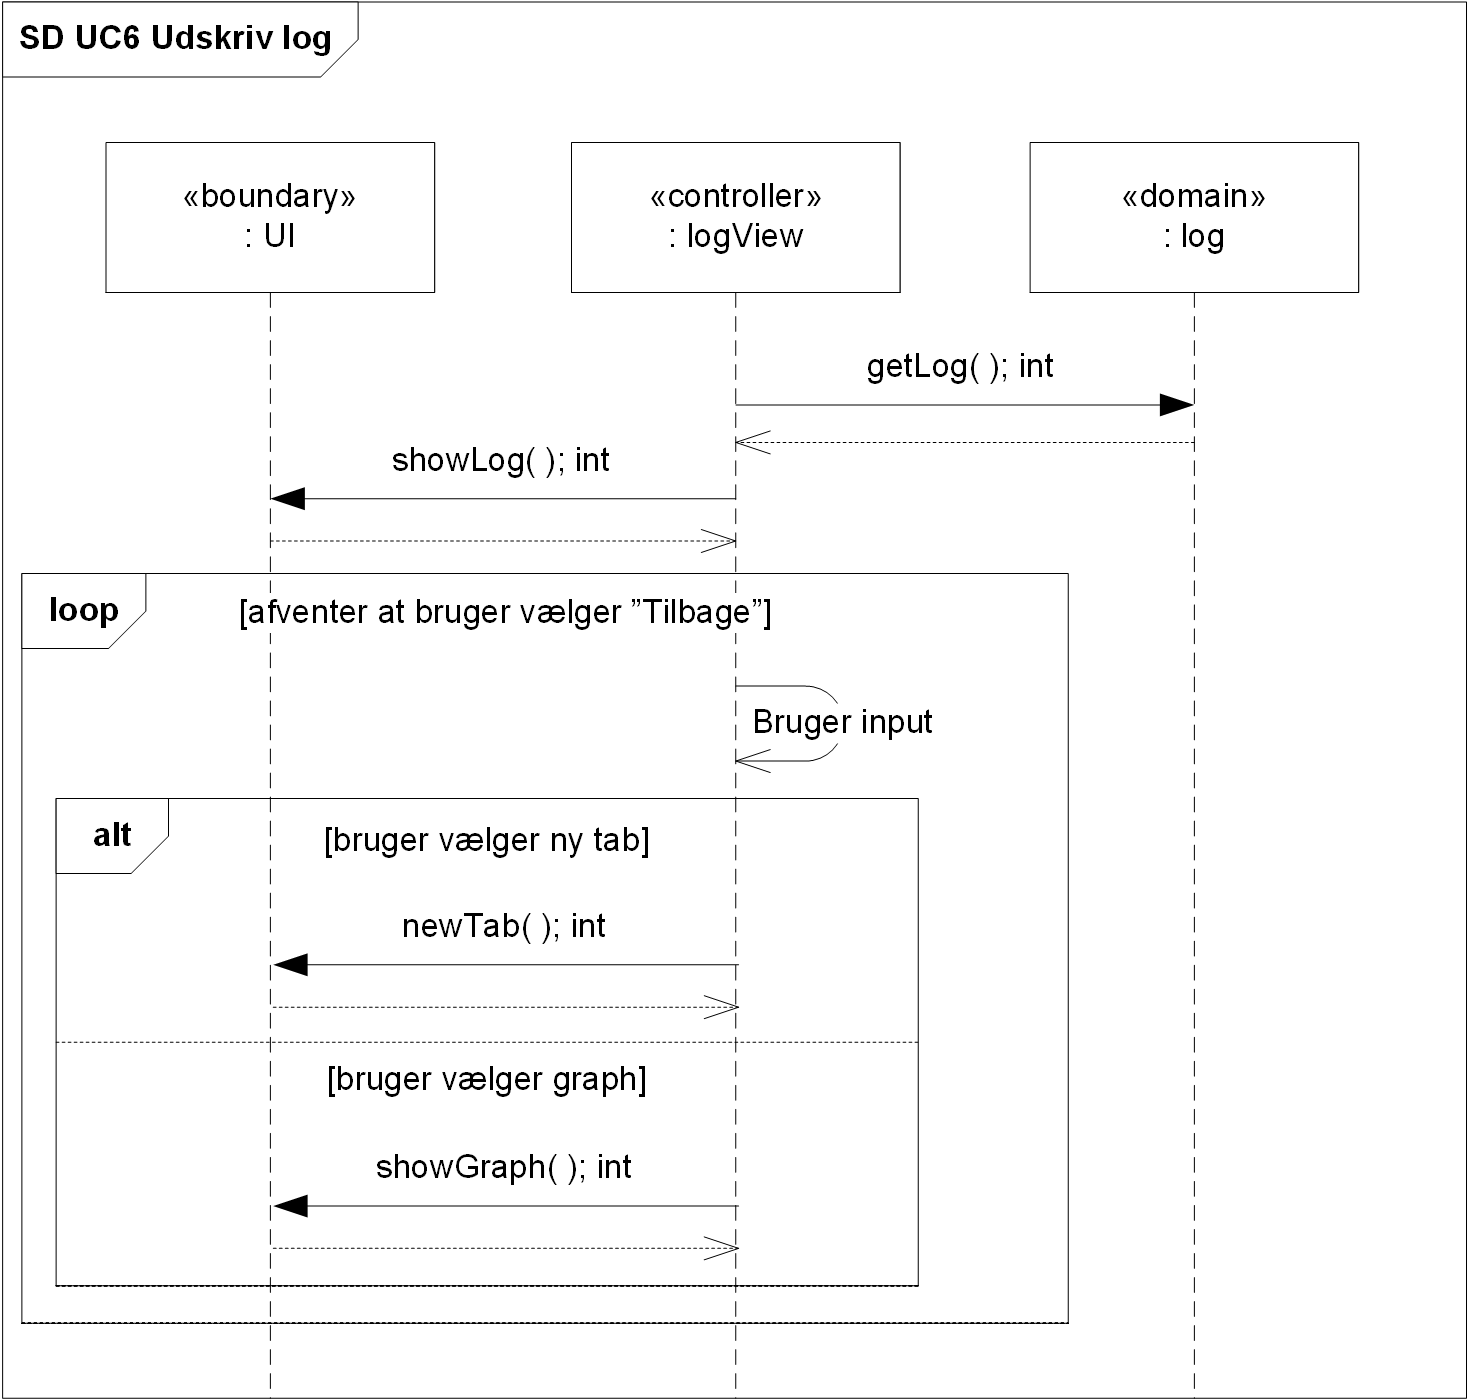
\includegraphics[scale=1]{filer/design/a_uc6}}
\caption{Sekvensdiagram UC6}
\label{fig:Sekvensdiagram UC6}
\end{figure} 

\clearpage
\begin{figure}[htbp] \centering
{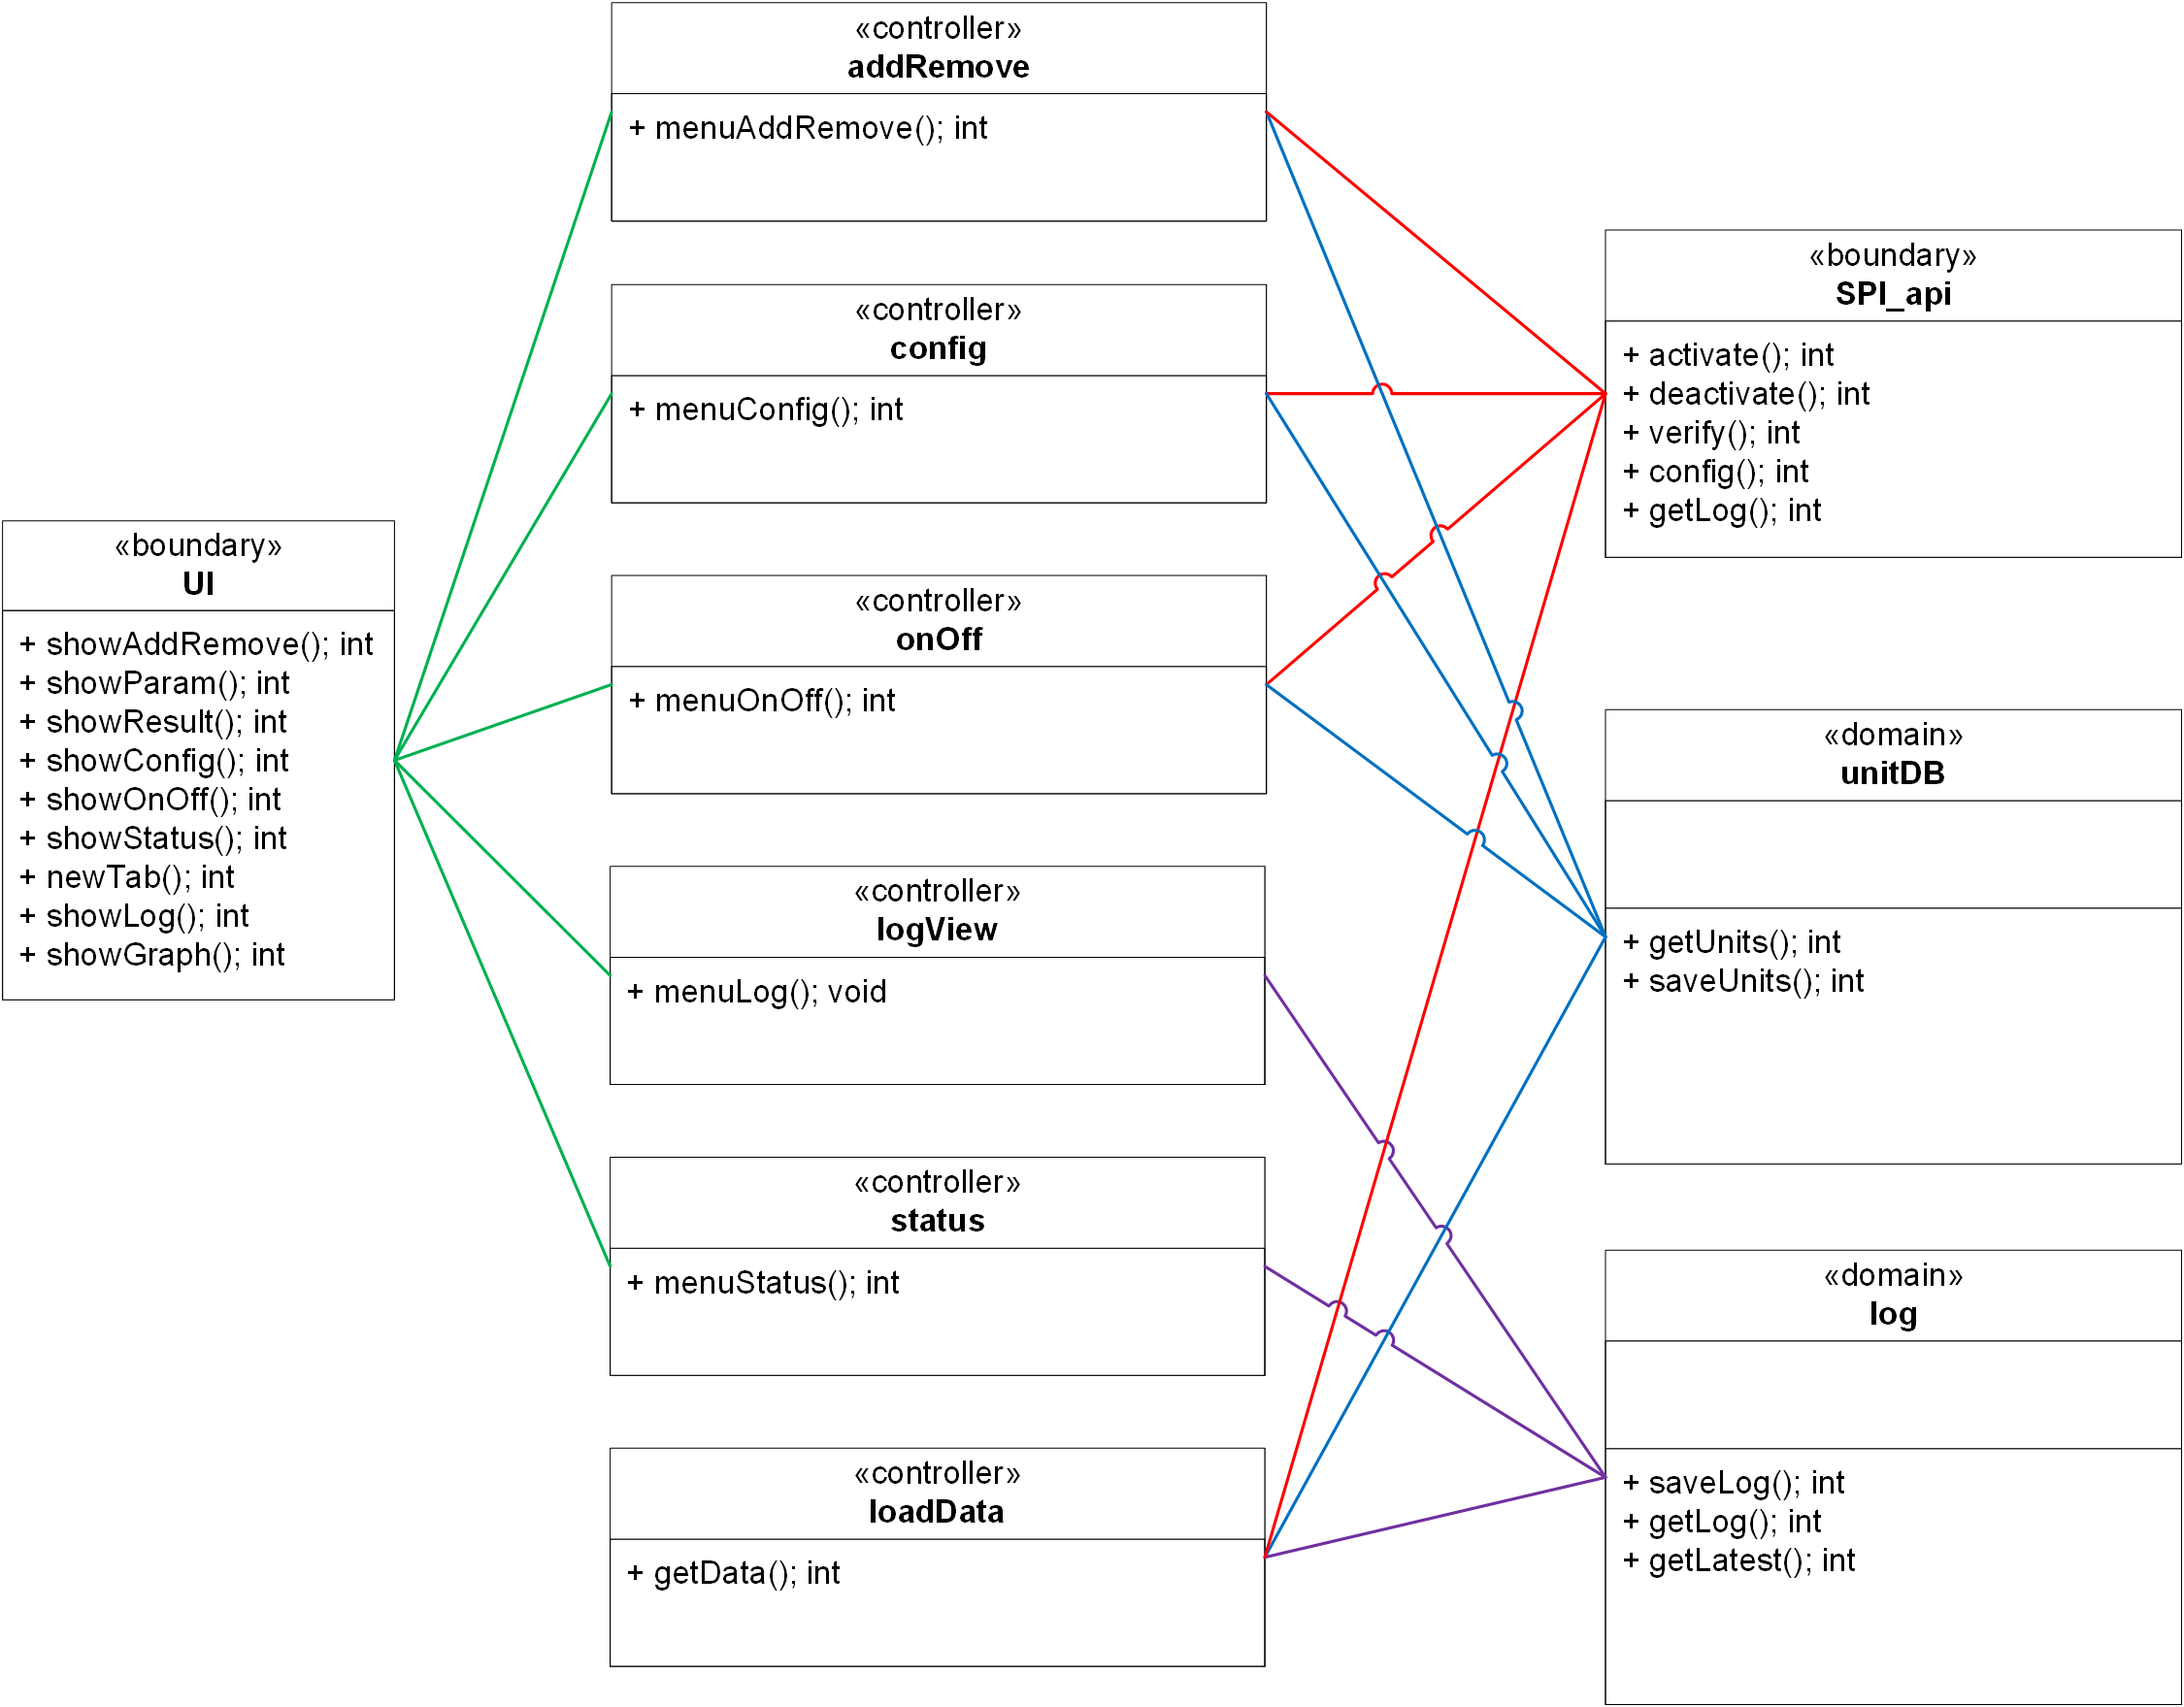
\includegraphics[scale=1]{filer/design/sw_class_devkit}}
\caption{klassediagram devkit8000}
\label{fig:klassediagram devkit8000}
\end{figure} 

Efter udarbejdelsen af sekvensdiagrammer samles alle metode kald imellem klasserne til et klassediagram som ses ovenfor på \ref{fig:klassediagram devkit8000}. Efter dette klassediagram udarbejdes en klassebeskrivelse hvor der tænkes over hvilke attributer de forskellige metoder skal have for at kunne udføre deres ansvar. Det bliver så fuldt op med et endeligt statisk klassediagram som inkludere alle attributer og medlems data.


\clearpage
\subsection{Enhed}
Applikationsmodeller for Enhed.

% Klassebeskrivelser
\subsection{Klassebeskrivelser}
Her følger klassebeskrivelser for de udledte klasser fra applikationsmodellerne.

% Master
\subsubsection{Master (JC)}
%% SW design: klassebeskrivelse SPI API

\begin{figure}[htbp] \centering
{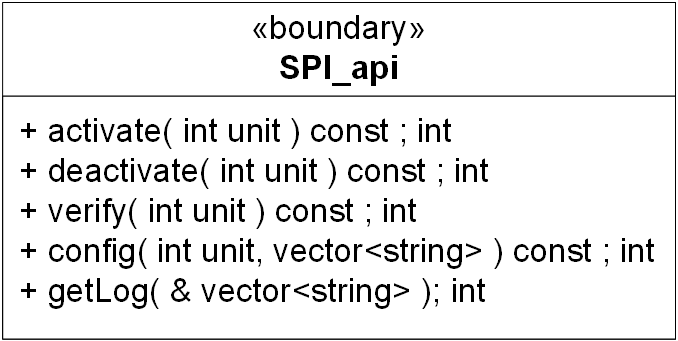
\includegraphics[scale=1.5]{filer/design/Klassediagrammer/SPI_API}}
\caption{klassediagram SPI API}
\label{fig:SPI API klassediagram}
\end{figure} 

{\centering
\textbf{SPI\_api klasse}\par
}
\textbf{Ansvar:} At være det lag imellem applications laget og device driver laget. Skal håndtere snakken med device driveren til SPI kommunikation \\

int activate( int unit ) const \\
\textbf{Parametre:} modtager en integer på følgende enhed som skal aktiveres \\
\textbf{Returværdi:} returnere en integer som er 0 hvis operationen gik godt. Ved fejl returneres en negativ integer i overenstemmelse med fejl-listen \\
\textbf{Beskrivelse:} metoden skal kunne aktivere enheden som er identificeret ved integeren den modtager. Hvis dette går godt returneres 0, ellers returneres en fejlkode i overenstemmelse med fejl-listen.\\

int deactivate( int unit ) const \\
\textbf{Parametre:}  modtager en integer på følgende enhed som skal deaktiveres\\
\textbf{Returværdi}: returnere en integer som er 0 hvis operationen gik godt. Ved fejl returneres en negativ integer i overenstemmelse med fejl-listen  \\
\textbf{Beskrivelse:} metoden skal kunne deaktivere enheden som er identificeret ved integeren den modtager. Hvis dette går godt returneres 0, ellers returneres en fejlkode i overenstemmelse med fejl-listen.\\

int verify( int unit ) const \\
\textbf{Parametre:}  modtager en integer på følgende enhed som skal verificerese\\
\textbf{Returværdi:} returnere en integer som er 0 hvis operationen gik godt. Ved fejl returneres en negativ integer i overenstemmelse med fejl-listen  \\
\textbf{Beskrivelse:} metoden skal kunne verificere om en enhed, identificeret ved integeren den modtager, er på SPI nettet. Hvis dette går godt returneres 0, ellers returneres en fejlkode i overenstemmelse med fejl-listen.\\

int config( int unit, vector<string> ) const \\
\textbf{Parametre:} modtager en integer på følgende enhed som skal konfigureres. Derudover modtager den en vector af typen string som indeholder parametrene enheden skal konfigureres med \\
\textbf{Returværdi:} returnere en integer som er 0 hvis operationen gik godt. Ved fejl returneres en negativ integer i overenstemmelse med fejl-listen  \\
\textbf{Beskrivelse:} metoden skal kunne sende konfigurations parametre ud til enheder ved hjælp af device driverne til SPI kommunikationen. Hvis dette går godt returneres 0, ellers returneres en fejlkode i overenstemmelse med fejl-listen.\\

int getLog( \& vector<string>  ) \\
\textbf{Parametre:}  modtager en referance til en vector af typen string som loggen skal lægges over i.\\
\textbf{Returværdi:} returnere en integer som er 0 hvis operationen gik godt. Ved fejl returneres en negativ integer i overenstemmelse med fejl-listen  \\
\textbf{Beskrivelse:} metoden skal kunne hente log fra alle enheder på SPI netværket og gemme dem i den modtaget vector. \\









%% SW design: klassebeskrivelse UI

\begin{figure}[htbp] \centering
{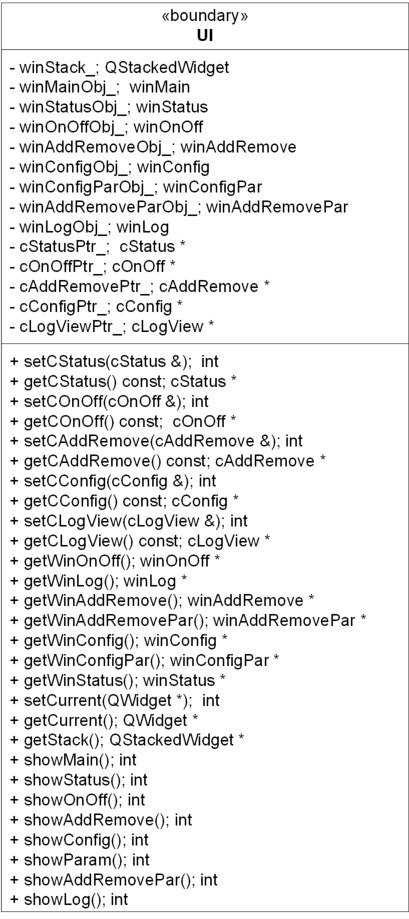
\includegraphics[scale=1.5]{filer/design/Klassediagrammer/sw_UI}}
\caption{Klasse UI}
\label{fig:UI klassediagram}
\end{figure} 

{\centering
\textbf{UI}\par
}
\textbf{Ansvar:} Håndterer alt ved den grafiske brugerflade. \

\textbf{Attributter:}
\begin{itemize}
	\item \verb+QStackedWidget winStack_+ Objekt til at holde alle vinduer i
	\item \verb+winMain winMainObj_+ Hovedmenu vindue
	\item \verb+winStatus winStatusObj_+ Vis status vindue
	\item \verb+winOnOff winOnOffObj_+ Aktiver / Deaktiver vindue
	\item \verb+winAddRemove winAddRemoveObj_+ Tilføj / fjern vindue
	\item \verb+winConfig winConfigObj_+ Konfigurer vindue
	\item \verb+winConfigPar winConfigParObj_+ Konfigurer parametre vindue
	\item \verb+winAddRemovePar winAddRemoveParObj_+ Tilføj Enheds parametre vindue
	\item \verb+winLog winLogObj_+ Vis Log vindue
	\item \verb+cStatus * cStatusPtr_+ Pointer til associeret objekt
	\item \verb+cOnOff * cOnOffPtr_+ Pointer til associeret objekt
	\item \verb+cAddRemove * cAddRemovePtr_+ Pointer til associeret objekt
	\item \verb+cConfig * cConfigPtr_+ Pointer til associeret objekt
	\item \verb+cLogView * cLogViewPtr_+ Pointer til associeret objekt
\end{itemize}

\verb+UI( )+\\
\textbf{Parametre:} Ingen \\
\textbf{Returværdi:} Ingen \\
\textbf{Beskrivelse:} Tilføjer alle \verb+win+-objekterne til stakken \verb+winStack_+. Sætter det aktive vindue til hovedmenuen \verb+winMainObj_+. Indstiller størrelsen på vinduer i stakken til at fylde hele skærmen på Devkit8000, 480x272 og sætter størrelsen på \verb+UI+ til at have samme størrelse. Til sidst opsættes den centrale widget i \verb+QMainWindow+ til stakken \verb+winStack_+.\\


\verb+int setCStatus( cStatus & )+\\
\textbf{Parametre:} Reference til associeret objekt \\
\textbf{Returværdi:} 0 ved succes ellers negativ i overenstemmelse med fejl-listen. \\
\textbf{Beskrivelse:} Sætter medlemspointer til associeret controller.\\

\verb+int setCOnOff( cOnOff & )+\\
\textbf{Parametre:} Reference til associeret objekt \\
\textbf{Returværdi:} 0 ved succes ellers negativ i overenstemmelse med fejl-listen. \\
\textbf{Beskrivelse:} Sætter medlemspointer til associeret controller.\\

\verb+int setCAddRemove( cAddRemove & )+\\
\textbf{Parametre:} Reference til associeret objekt \\
\textbf{Returværdi:} 0 ved succes ellers negativ i overenstemmelse med fejl-listen. \\
\textbf{Beskrivelse:} Sætter medlemspointer til associeret controller.\\

\verb+int setCConfig( cConfig & )+\\
\textbf{Parametre:} Reference til associeret objekt \\
\textbf{Returværdi:} 0 ved succes ellers negativ i overenstemmelse med fejl-listen. \\
\textbf{Beskrivelse:} Sætter medlemspointer til associeret controller.\\

\verb+int setCLogView( cLogView & )+\\
\textbf{Parametre:} Reference til associeret objekt \\
\textbf{Returværdi:} 0 ved succes ellers negativ i overenstemmelse med fejl-listen. \\
\textbf{Beskrivelse:} Sætter medlemspointer til associeret controller.\\

\verb+cStatus * getCStatus( ) const+\\
\textbf{Parametre:} Ingen \\
\textbf{Returværdi:} 0 ved succes ellers negativ i overenstemmelse med fejl-listen. \\
\textbf{Beskrivelse:} Returnerer pointer til associeret objekt.\\

\verb+cOnOff * getCOnOff( ) const+\\
\textbf{Parametre:} Ingen \\
\textbf{Returværdi:} 0 ved succes ellers negativ i overenstemmelse med fejl-listen. \\
\textbf{Beskrivelse:} Returnerer pointer til associeret objekt.\\

\verb+cAddRemove * getCAddRemove( ) const+\\
\textbf{Parametre:} Ingen \\
\textbf{Returværdi:} 0 ved succes ellers negativ i overenstemmelse med fejl-listen. \\
\textbf{Beskrivelse:} Returnerer pointer til associeret objekt.\\

\verb+cConfig * getCConfig( ) const+\\
\textbf{Parametre:} Ingen \\
\textbf{Returværdi:} 0 ved succes ellers negativ i overenstemmelse med fejl-listen. \\
\textbf{Beskrivelse:} Returnerer pointer til associeret objekt.\\

\verb+cLogView * getCLogView( ) const+\\
\textbf{Parametre:} Ingen \\
\textbf{Returværdi:} 0 ved succes ellers negativ i overenstemmelse med fejl-listen. \\
\textbf{Beskrivelse:} Returnerer pointer til associeret objekt.\\

\verb+winOnOff * getWinOnOff( )+\\
\textbf{Parametre:} Ingen \\
\textbf{Returværdi:} 0 ved succes ellers negativ i overenstemmelse med fejl-listen. \\
\textbf{Beskrivelse:} Returnerer pointer til associeret objekt.\\

\verb+winLog * getWinLog( )+\\
\textbf{Parametre:} Ingen \\
\textbf{Returværdi:} 0 ved succes ellers negativ i overenstemmelse med fejl-listen. \\
\textbf{Beskrivelse:} Returnerer pointer til associeret objekt.\\

\verb+winAddRemove * getWinAddRemove( )+\\
\textbf{Parametre:} Ingen \\
\textbf{Returværdi:} 0 ved succes ellers negativ i overenstemmelse med fejl-listen. \\
\textbf{Beskrivelse:} Returnerer pointer til associeret objekt.\\

\verb+winAddRemovePar * getWinAddRemovePar( )+\\
\textbf{Parametre:} Ingen \\
\textbf{Returværdi:} 0 ved succes ellers negativ i overenstemmelse med fejl-listen. \\
\textbf{Beskrivelse:} Returnerer pointer til associeret objekt.\\

\verb+winConfig * getWinConfig( )+\\
\textbf{Parametre:} Ingen \\
\textbf{Returværdi:} 0 ved succes ellers negativ i overenstemmelse med fejl-listen. \\
\textbf{Beskrivelse:} Returnerer pointer til associeret objekt.\\

\verb+winConfigPar * getWinConfigPar( )+\\
\textbf{Parametre:} Ingen \\
\textbf{Returværdi:} 0 ved succes ellers negativ i overenstemmelse med fejl-listen. \\
\textbf{Beskrivelse:} Returnerer pointer til associeret objekt.\\

\verb+winStatus * getWinStatus( )+\\
\textbf{Parametre:} Ingen \\
\textbf{Returværdi:} 0 ved succes ellers negativ i overenstemmelse med fejl-listen. \\
\textbf{Beskrivelse:} Returnerer pointer til associeret objekt.\\

\verb+int setCurrent(QWidget *)+\\
\textbf{Parametre:} Pointer til vindue som skal vises i stakken. \\
\textbf{Returværdi:} 0 ved succes ellers negativ i overenstemmelse med fejl-listen. \\
\textbf{Beskrivelse:} LADER IKKE TIL AT VÆRE IMPLEMENTERET???.\\

\verb+QWidget * getCurrent( )+\\
\textbf{Parametre:} Ingen \\
\textbf{Returværdi:} 0 ved succes ellers negativ i overenstemmelse med fejl-listen. \\
\textbf{Beskrivelse:} LADER IKKE TIL AT VÆRE IMPLEMENTERET???.\\

\verb+QStackedWidget * getStack( )+\\
\textbf{Parametre:} Ingen \\
\textbf{Returværdi:} 0 ved succes ellers negativ i overenstemmelse med fejl-listen. \\
\textbf{Beskrivelse:} Returnerer pointer til winStack-objektet.\\

\verb+int showMain( )+\\
\textbf{Parametre:} Ingen \\
\textbf{Returværdi:} 0 ved succes ellers negativ i overenstemmelse med fejl-listen. \\
\textbf{Beskrivelse:} Sætter aktive vindue i \verb+winStack_+-objektet til \verb+winMainObj_+.\\

\verb+int showStatus( )+\\
\textbf{Parametre:} Ingen \\
\textbf{Returværdi:} 0 ved succes ellers negativ i overenstemmelse med fejl-listen. \\
\textbf{Beskrivelse:} Sætter aktive vindue i \verb+winStack_+-objektet til \verb+winStatusObj_+.\\

\verb+int showOnOff( )+\\
\textbf{Parametre:} Ingen \\
\textbf{Returværdi:} 0 ved succes ellers negativ i overenstemmelse med fejl-listen. \\
\textbf{Beskrivelse:} Sætter aktive vindue i \verb+winStack_+-objektet til \verb+winOnOffObj_+.\\

\verb+int showAddRemove( )+\\
\textbf{Parametre:} Ingen \\
\textbf{Returværdi:} 0 ved succes ellers negativ i overenstemmelse med fejl-listen. \\
\textbf{Beskrivelse:} Sætter aktive vindue i \verb+winStack_+-objektet til \verb+winAddRemoveObj_+.\\

\verb+int showConfig( )+\\
\textbf{Parametre:} Ingen \\
\textbf{Returværdi:} 0 ved succes ellers negativ i overenstemmelse med fejl-listen. \\
\textbf{Beskrivelse:} Sætter aktive vindue i \verb+winStack_+-objektet til \verb+winConfigObj_+.\\

\verb+int showParam( )+\\
\textbf{Parametre:} Ingen \\
\textbf{Returværdi:} 0 ved succes ellers negativ i overenstemmelse med fejl-listen. \\
\textbf{Beskrivelse:} Sætter aktive vindue i \verb+winStack_+-objektet til \verb+winConfigParObj_+.\\

\verb+int showAddRemovePar( )+\\
\textbf{Parametre:} Ingen \\
\textbf{Returværdi:} 0 ved succes ellers negativ i overenstemmelse med fejl-listen. \\
\textbf{Beskrivelse:} Sætter aktive vindue i \verb+winStack_+-objektet til \verb+winAddRemoveParObj_+.\\

\verb+int showLog( )+\\
\textbf{Parametre:} Ingen \\
\textbf{Returværdi:} 0 ved succes ellers negativ i overenstemmelse med fejl-listen. \\
\textbf{Beskrivelse:} Sætter aktive vindue i \verb+winStack_+-objektet til \verb+winLogObj_+.\\


%% SW design: klassebeskrivelse devkit Controllers
\newpage

\begin{figure}[htbp] \centering
{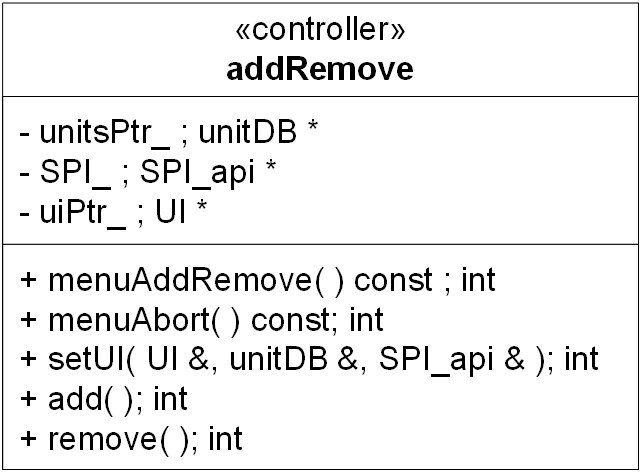
\includegraphics[scale=1.5]{filer/design/Klassediagrammer/sw_addRemove}}
\caption{klassediagram addRemove}
\label{fig:addRemove klassediagram}
\end{figure} 

{\centering
\textbf{addRemove}\par
}
\textbf{Ansvar:} at styre forløbet i UC1: Tilføj / fjern enhed. \

\verb+int menuAddRemove( ) const+ \\
\textbf{Parametre:} Modtager ingen parametre \\
\textbf{Returværdi:} 0 ved succes ellers negativ i overenstemmelse med fejl-listen \\
\textbf{Beskrivelse:} Modtager information fra brugeren omkring enhed, verificere enheden over SPI netværket og gemme information i databasen..\\

\begin{figure}[htbp] \centering
{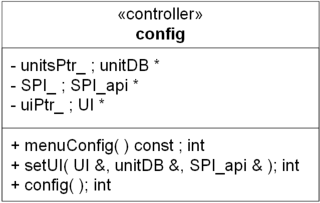
\includegraphics[scale=1.5]{filer/design/Klassediagrammer/sw_config}}
\caption{klassediagram config}
\label{fig:config klassediagram}
\end{figure} 

{\centering
\textbf{Config}\par
}
\textbf{Ansvar:} at styre forløbet i UC2: Konfig. \

\verb+int menuConfig( ) const+ \\
\textbf{Parametre:} Modtager ingen parametre \\
\textbf{Returværdi:} 0 ved succes ellers negativ i overenstemmelse med fejl-listen \\
\textbf{Beskrivelse:} Modtager information fra brugeren omkring enhed og parametre. Parametrene skrives til den pågældende enhed på SPI netværket.\\

\begin{figure}[htbp] \centering
{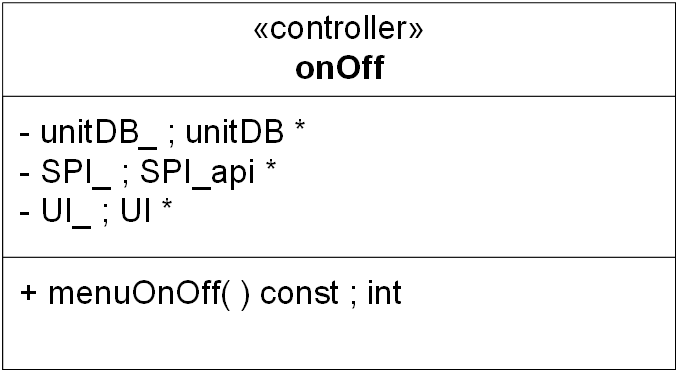
\includegraphics[scale=1.5]{filer/design/Klassediagrammer/sw_onOff}}
\caption{klassediagram onOff}
\label{fig:onOff klassediagram}
\end{figure} 

\newpage

{\centering
\textbf{onOff}\par
}
\textbf{Ansvar:} at styre forløbet i UC3: Aktiver / deaktiver. \

\verb+int menuOnOff( ) const+ \\
\textbf{Parametre:} Modtager ingen parametre \\
\textbf{Returværdi:} 0 ved succes ellers negativ i overenstemmelse med fejl-listen \\
\textbf{Beskrivelse:} Modtager information fra brugeren omkring hvilken enhed som ønskes aktiveret eller deaktiveret. Enheden modtager informationen over SPI netværket.\\

\begin{figure}[htbp] \centering
{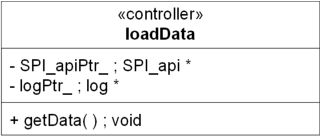
\includegraphics[scale=1.5]{filer/design/Klassediagrammer/sw_loadData}}
\caption{klassediagram loadData}
\label{fig:loadData klassediagram}
\end{figure} 

{\centering
\textbf{loadData}\par
}
\textbf{Ansvar:} at styre forløbet i UC4: Databehandling . \

\verb+void getData( )+ \\
\textbf{Parametre:} Modtager ingen parametre \\
\textbf{Returværdi:} 0 ved succes ellers negativ i overenstemmelse med fejl-listen \\
\textbf{Beskrivelse:} Kaldes af en uafhængig tråd når en timer løber ud. Skal hente log-data over SPI netværket. Kontrollerer om der er nogle sensor-læsninger i mellem dataen og gemme denne i \verb+log+-objektet. Fejl gemmes ikke i \verb+log+.\\

\begin{figure}[htbp] \centering
{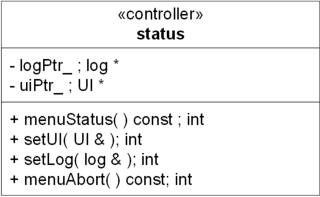
\includegraphics[scale=1.5]{filer/design/Klassediagrammer/sw_status}}
\caption{klassediagram status}
\label{fig:status klassediagram}
\end{figure} 

\newpage

{\centering
\textbf{status}\par
}
\textbf{Ansvar:} at styre forløbet i UC5: Tjek status. \

\verb+int menuStatus( ) const+ \\
\textbf{Parametre:} Modtager ingen parametre \\
\textbf{Returværdi:} 0 ved succes ellers negativ i overenstemmelse med fejl-listen \\
\textbf{Beskrivelse:} Henter den seneste log i hukommelsen og viser brugeren den, for den ønskede enhed.\\

\begin{figure}[htbp] \centering
{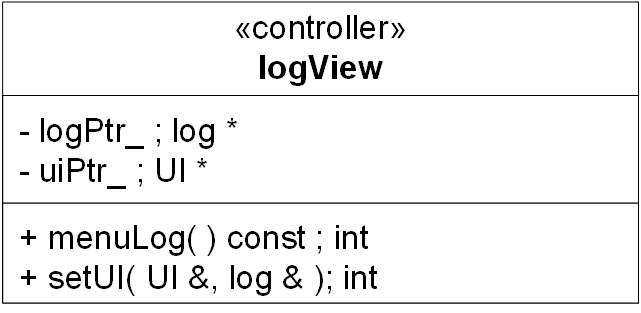
\includegraphics[scale=1.5]{filer/design/Klassediagrammer/sw_logView}}
\caption{klassediagram logView}
\label{fig:logView klassediagram}
\end{figure}

{\centering
\textbf{logView}\par
}
\textbf{Ansvar:} at styre forløbet i UC6: Udskriv log. \

\verb+int menuLog( ) const+ \\
\textbf{Parametre:} Modtager ingen parametre \\
\textbf{Returværdi:} 0 ved succes ellers negativ i overenstemmelse med fejl-listen \\
\textbf{Beskrivelse:} Henter hele loggen i hukommelsen og viser brugeren den, for den ønskede enhed.\\


%% SW design: klassebeskrivelse devkit domain klasser
\newpage

\begin{figure}[htbp] \centering
{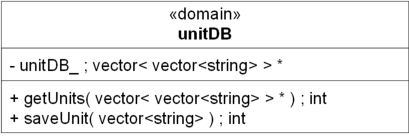
\includegraphics[scale=1.5]{filer/design/Klassediagrammer/sw_unitDB}}
\caption{Klasse unitDB}
\label{fig:unitDB klassediagram}
\end{figure} 

{\centering
\textbf{unitDB}\par
}
\textbf{Ansvar:} Gemmer opsatte Enheder og deres parametre. \

\textbf{Attributter:}
\begin{itemize}
	\item \verb+vector< vector<string> > * unitDB_+ Dynamisk allokeret \verb+vector+ til enhedsliste.
\end{itemize}

\verb+unitDB( ) +\\
\textbf{Parametre:} Ingen.\\
\textbf{Returværdi:} Ingen. \\
\textbf{Beskrivelse:} Allokerer dynamisk en \verb+vector< vector<string> >+ til attributten \verb+unitDB_+. Indsætter 18 enheder af typen \verb+vector<string>+ med grænserne -1 for temperatur og fugtighed, og status sættes til [Deaktiv] på hhv. index 1, 2, 3. Index 0 er nummeret på enheden. \\

\verb+~unitDB( ) +\\
\textbf{Parametre:} Ingen.\\
\textbf{Returværdi:} Ingen. \\
\textbf{Beskrivelse:} Deallokerer \verb+unitDB_+. \\

\verb+int getUnits( vector< vector<string> > * ) +\\
\textbf{Parametre:} Modtager pointer til hvor enhedslisten skal gemmes.\\
\textbf{Returværdi:} 0 ved succes ellers negativ i overenstemmelse med fejl-listen. \\
\textbf{Beskrivelse:} Skriver indholdet af \verb+unitDB_+ over i den modtagne pointer. \\

\verb+int saveUnit( vector<string> ) +\\
\textbf{Parametre:} \verb+vector+ som skal gemmes \\
\textbf{Returværdi:} 0 ved succes ellers negativ i overenstemmelse med fejl-listen. \\
\textbf{Beskrivelse:} Finder enhedsnummer fra modtagne vektor og gemmer data i den pågældende plads i \verb+unitDB_+. \\

\begin{figure}[htbp] \centering
{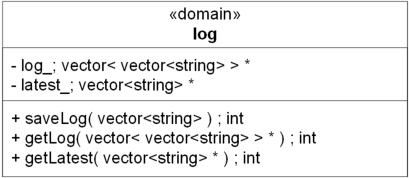
\includegraphics[scale=1.5]{filer/design/Klassediagrammer/sw_log}}
\caption{Klasse log}
\label{fig:log klassediagram}
\end{figure} 

{\centering
\textbf{log}\par
}
\textbf{Ansvar:} Gemmer log-information fra tilkoblede Enheder. \

\textbf{Attributter:}
\begin{itemize}
	\item \verb+vector< vector<string> > * log_+ Dynamisk allokeret \verb+vector+ til loggen.
	\item \verb+vector<string> * latest_+ Dynamisk allokeret \verb+vector+ til senest loggede information.
\end{itemize}

\verb+log( ) +\\
\textbf{Parametre:} Ingen \\
\textbf{Returværdi:} Ingen\\
\textbf{Beskrivelse:} Allokerer dynamisk en \verb+vector< vector<string> >+ til \verb+log_+ og en \verb+vector<string>+ til \verb+latest_+. \\

\verb+~log( ) +\\
\textbf{Parametre:} Ingen \\
\textbf{Returværdi:} Ingen\\
\textbf{Beskrivelse:} Deallokerer \verb+log_+ og \verb+latest_+. \\

\verb+int saveLog( vector<string> ) +\\
\textbf{Parametre:} \verb+vector+ som skal gemmes. \\
\textbf{Returværdi:} 0 ved succes ellers negativ i overenstemmelse med fejl-listen. \\
\textbf{Beskrivelse:} Gemmer modtaget data ved at pushe \verb+log_+ og overskrive \verb+latest+. \\

\verb+int getLog( vector< vector<string> > * ) + \\
\textbf{Parametre:} Pointer til hvor data skal gemmes. \\
\textbf{Returværdi:} 0 ved succes ellers negativ i overenstemmelse med fejl-listen. \\
\textbf{Beskrivelse:} Skriver data fra \verb+log_+ over i modtagne pointer. \\

\verb+int getLatest( vector<string> * ) +\\
\textbf{Parametre:} Pointer til hvor data skal gemmes.  \\
\textbf{Returværdi:} 0 ved succes ellers negativ i overenstemmelse med fejl-listen. \\
\textbf{Beskrivelse:} Skriver data fra \verb+latest_+ over i modtagne pointer. \\




% Enhed
\subsubsection{Enhed (BS)}
Her følger klassebeskrivelser til Enhed. 
Bemærk at alt kode til PSoC er skrevet i \verb+C+, hvorfor det ikke er muligt at lave klasser. Beskrivelserne tager dog udgangspunkt i \verb-C++-, men skal fortolkes iht. beskrivelsen i \textit{UML-Light}\footnote{T-133 UML-Light af Finn Overgaard Hansen. Benyttet i forbindelse med faget I1OPRG (Objektorienteret PRoGrammering) på 1. semester.} 

%% SW design: PSoC Controllers

\begin{figure}[htbp] \centering
{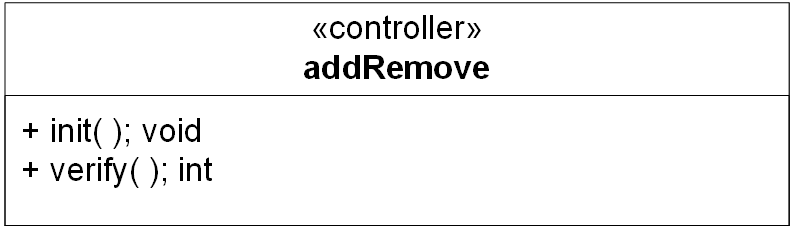
\includegraphics[scale=1.3]{filer/design/Klassediagrammer/sw_psoc_addRemove}}
\caption{Klasse addRemove}
\label{fig:sw_psoc_class_addremove}
\end{figure} 

{\centering
\textbf{addRemove}\par
}
\textbf{Ansvar:} Kontrollerer hændelsesforløbet ifm. usecase 1. \

\verb+int verify( ) const +\\
\textbf{Parametre:} Ingen \\
\textbf{Returværdi:} 0 ved succes ellers negativ i overenstemmelse med fejl-listen. \\
\textbf{Beskrivelse:} Returnerer kun 0. Bruges til at verificerer kommunikation mellem Master og Enhed.\\

\begin{figure}[htbp] \centering
{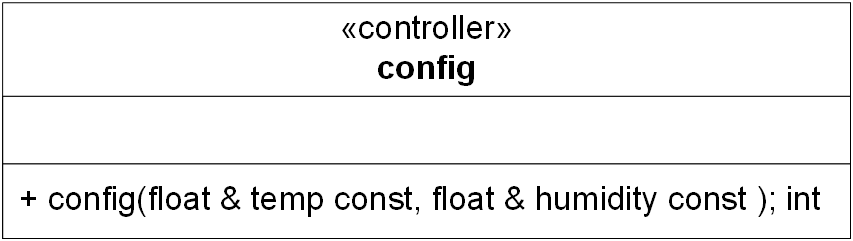
\includegraphics[scale=1.3]{filer/design/Klassediagrammer/sw_psoc_config}}
\caption{Klasse config}
\label{fig:sw_psoc_class_config}
\end{figure} 

{\centering
\textbf{config}\par
}
\textbf{Ansvar:} Kontrollerer hændelsesforløbet ifm. usecase 2. \

\verb+int config( float & temp const, float & humidity const )+ \\
\textbf{Parametre:} To referencer til hhv. temperatur og fugtighedsgrænser \\
\textbf{Returværdi:} 0 ved succes ellers negativ i overenstemmelse med fejl-listen. \\
\textbf{Beskrivelse:} Skal gemme parametre i et objekt af typen parameters.\\

\begin{figure}[htbp] \centering
{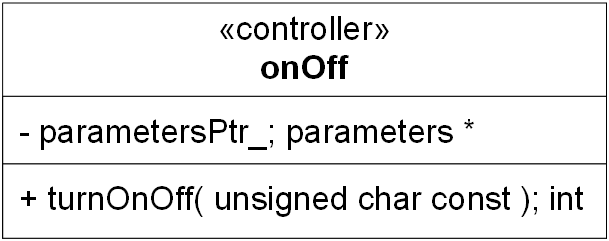
\includegraphics[scale=1.3]{filer/design/Klassediagrammer/sw_psoc_onOff}}
\caption{Klasse onOff}
\label{fig:sw_psoc_class_onOff}
\end{figure} 

{\centering
\textbf{onOff}\par
}
\textbf{Ansvar:} Kontrollerer hændelsesforløbet ifm. usecase 3. \

\verb+int turnOnOff( bool onOff const )+ \\
\textbf{Parametre:} En \verb+bool+ som angiver on = true, off = false \\
\textbf{Returværdi:} 0 ved succes ellers negativ i overenstemmelse med fejl-listen. \\
\textbf{Beskrivelse:} Skal sætte flaget \verb+active_+ i \verb+parameters+-objektet ud fra den modtagende parameter.\\

\begin{figure}[htbp] \centering
{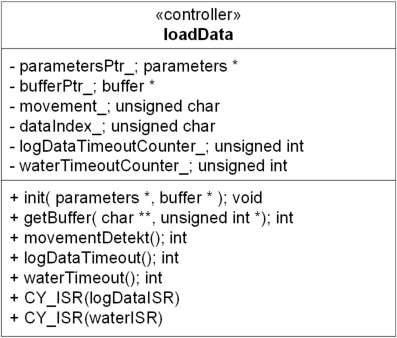
\includegraphics[scale=1.3]{filer/design/Klassediagrammer/sw_psoc_loadData}}
\caption{Klasse loadData}
\label{fig:sw_psoc_class_loadData}
\end{figure} 

{\centering
\textbf{loadData}\par
}
\textbf{Ansvar:} Kontrollerer hændelsesforløbet ifm. usecase 4. \

\verb+int getBuffer( vector<string> & buf )+ \\
\textbf{Parametre:} En reference til en skrivbar buffer \\
\textbf{Returværdi:} 0 ved succes ellers negativ i overenstemmelse med fejl-listen. \\
\textbf{Beskrivelse:} Skal hente data fra \verb+buffer+-objektet og gemme det i parametren buf.\\

\verb+int movementDetekt( )+ \\
\textbf{Parametre:} Ingen. \\
\textbf{Returværdi:} 0 ved succes ellers negativ i overenstemmelse med fejl-listen. \\
\textbf{Beskrivelse:} Skal deaktiverer vanding ved at sætte \verb+active_+-flaget i \verb+parameters+-objektet til 0. Skal også starte en timer som ved udløbet skal aktiverer vandingen igen efter 30 minutter.\\
%% SW design: PSoC Domain

\begin{figure}[htbp] \centering
{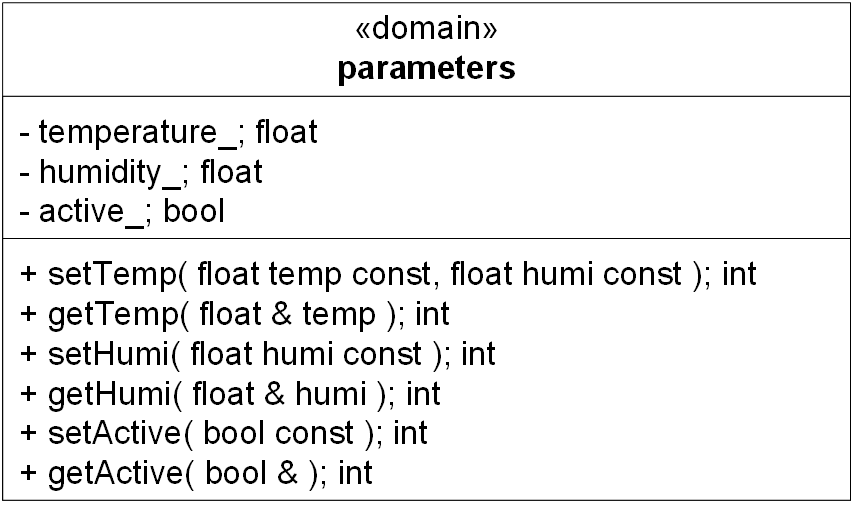
\includegraphics[scale=1.3]{filer/design/Klassediagrammer/sw_psoc_parameters}}
\caption{Klasse parameters}
\label{fig:sw_psoc_class_parameters}
\end{figure} 

{\centering
\textbf{parameters}\par
}
\textbf{Ansvar:} Gemme information om grænseværdier mv. til det autonome vandingssystem. \

\verb+int setTemp( float temp const ) +\\
\textbf{Parametre:} temperatur. \\
\textbf{Returværdi:} 0 ved succes ellers negativ i overenstemmelse med fejl-listen. \\
\textbf{Beskrivelse:} Gemmer modtagne temperatur i medlemsdata \verb+temperature_+. \\

\verb+int getTemp( float * temp )+ \\
\textbf{Parametre:} Pointer til at gemme temperatur i. \\
\textbf{Returværdi:} 0 ved succes ellers negativ i overenstemmelse med fejl-listen. \\
\textbf{Beskrivelse:} Returnerer medlem \verb+temperature_+ i reference. \\

\verb+int setHumi( float humi const )+ \\
\textbf{Parametre:} humidity. \\
\textbf{Returværdi:} 0 ved succes ellers negativ i overenstemmelse med fejl-listen. \\
\textbf{Beskrivelse:} Gemmer modtagne humidity i medlemsdata \verb+humidity_+. \\

\verb+int getHumi( float * humi )+ \\
\textbf{Parametre:} Pointer til at gemme humidity i. \\
\textbf{Returværdi:} 0 ved succes ellers negativ i overenstemmelse med fejl-listen. \\
\textbf{Beskrivelse:} Returnerer medlem \verb+humidity_+ i reference. \\

\verb+int setActive( unsigned char const )+ \\
\textbf{Parametre:} 1 = aktiv, 0 = inaktiv. \\
\textbf{Returværdi:} 0 ved succes ellers negativ i overenstemmelse med fejl-listen. \\
\textbf{Beskrivelse:} Gemmer modtagne char i medlemsdata \verb+active_+. \\

\verb+int getActive( unsigned char * )+ \\
\textbf{Parametre:} Pointer til at gemme unsigned char i. \\
\textbf{Returværdi:} 0 ved succes ellers negativ i overenstemmelse med fejl-listen. \\
\textbf{Beskrivelse:} Returnerer medlem \verb+active_+ i pointer. \\


\begin{figure}[htbp] \centering
{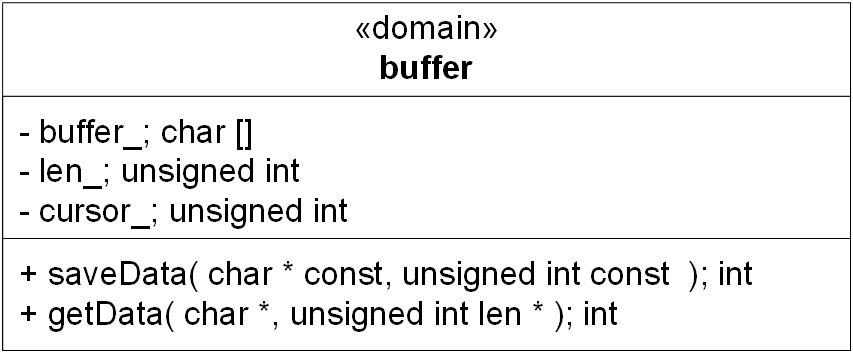
\includegraphics[scale=1.3]{filer/design/Klassediagrammer/sw_psoc_buffer}}
\caption{Klasse buffer}
\label{fig:sw_psoc_class_buffer}
\end{figure} 

{\centering
\textbf{buffer}\par
}
\textbf{Ansvar:} Holde data fra sensorerne indtil de udlæses af Master \

\verb+buffer( )+ \\
\textbf{Parametre:} Ingen. \\
\textbf{Returværdi:} Ingen. \\
\textbf{Beskrivelse:} Skal initialisere \verb+char+ array \verb+buffer_+ med plads til én datamåling og 10 fejl iht. dataprotokol. \\

\verb+int saveData( char * buf const, unsigned int len const )+ \\
\textbf{Parametre:} Pointer til buffer med len data. \\
\textbf{Returværdi:} 0 ved succes ellers negativ i overenstemmelse med fejl-listen. \\
\textbf{Beskrivelse:} Skal gemme modtaget data i \verb+buffer_+-medlemmet og flytte \verb+cursor_+ antallet af karakterer frem.\\

\verb+int getData( char * buf, unsigned int len )+ \\
\textbf{Parametre:} Pointer til char array til data. \\
\textbf{Returværdi:} 0 ved succes ellers negativ i overenstemmelse med fejl-listen. \\
\textbf{Beskrivelse:} Skal returnerer data fra \verb+buffer_+ i pointer og nulstille \verb+cursor_+-medlemmet.\\
%% SW design: PSoC Boundary

\begin{figure}[htbp] \centering
{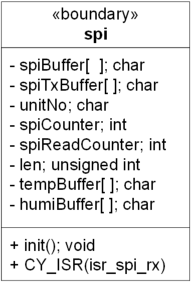
\includegraphics[scale=1.3]{filer/design/Klassediagrammer/sw_psoc_SPIhandler}}
\caption{Klasse spi}
\label{fig:sw_psoc_class_spi}
\end{figure} 

{\centering
\textbf{spi}\par
}
\textbf{Ansvar:} Håndterer kommunikation i mellem Master og Enhed. \

\textbf{Attributter:}
\begin{itemize}
	\item \verb+char spiBuffer[]+ Bruges til modtagede SPI kommandoer fra Master
	\item \verb+char spiTxBuffer[]+ Bruges til afsendelse af SPI kommandoer til Master
	\item \verb+char unitNo+ Enheds nummer til verificering
	\item \verb+int spiCounter+ Tæller til antallet af modtagne data-stykker
	\item \verb+int spiReadCounter+ Tæller til antallet af afsendte data-stykker
	\item \verb+unsigned int len+ Længde til afsendelse af log-data
	\item \verb+char tempBuffer[]+ Midlertidig buffer til konfigurering af parametre
	\item \verb+char humiBuffer[]+ Midlertidig buffer til konfigurering af parametre
\end{itemize}

\verb+void init( ) +\\
\textbf{Parametre:} Ingen. \\
\textbf{Returværdi:} Ingen. \\
\textbf{Beskrivelse:} Starter \verb+SPIS_1+ komponenten, sætter ISR-callback funktionen til \verb+isr_spi_rx+ og nulstiler RX bufferen. \\

\verb+CY_ISR(isr_spi_rx) +\\
\textbf{Parametre:} Ingen. \\
\textbf{Returværdi:} Ingen. \\
\textbf{Beskrivelse:} Læser modtaget data og kalder de aktuelle controller-klasser. \\

\begin{figure}[htbp] \centering
{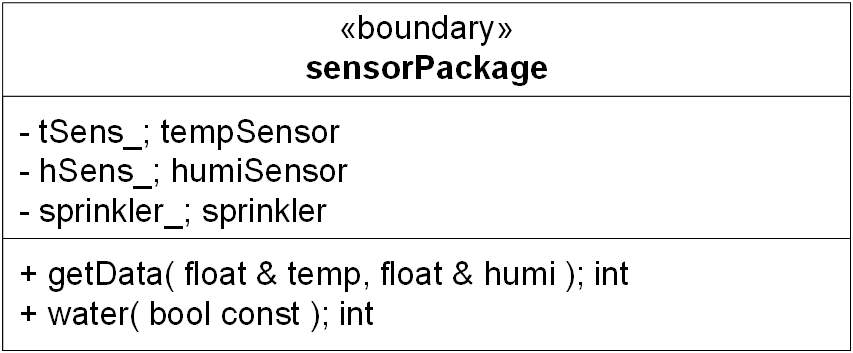
\includegraphics[scale=1.3]{filer/design/Klassediagrammer/sw_psoc_sensorPackage}}
\caption{Klasse sensorPackage}
\label{fig:sw_psoc_class_sensorPackage}
\end{figure} 

{\centering
\textbf{sensorPackage}\par
}
\textbf{Ansvar:} Holder styr på tilkoblede sensorer. \

\verb+void init( ) +\\
\textbf{Parametre:} Ingen. \\
\textbf{Returværdi:} Ingen. \\
\textbf{Beskrivelse:} Starter \verb+ADC_SAR_Seq_0+ og initialiserer tilkoblede sensorer og sprinkler ved at kalde deres \verb+init()+-metoder. \\

\verb+void exit( ) +\\
\textbf{Parametre:} Ingen. \\
\textbf{Returværdi:} Ingen. \\
\textbf{Beskrivelse:} Stopper \verb+ADC_SAR_Seq_0+. \\

\verb+int getData( float * temp, float * humi )+ \\
\textbf{Parametre:} Pointere til at gemme aflæste temperatur og fugtighed i. \\
\textbf{Returværdi:} 0 ved succes ellers negativ i overenstemmelse med fejl-listen. \\
\textbf{Beskrivelse:} Aflæser data fra temperatur- og fugtighedssensor og returnere disse i de modtagende pointere. \\

\verb+int water( const unsigned char )+ \\
\textbf{Parametre:} 1 = tænd sprinkler, 0 = sluk sprinkler. \\
\textbf{Returværdi:} 0 ved succes ellers negativ i overenstemmelse med fejl-listen. \\
\textbf{Beskrivelse:} Tænd eller sluk tilkoblede sprinkler ud fra modtagende parameter på komponent \verb+P_VP+. \\


\begin{figure}[htbp] \centering
{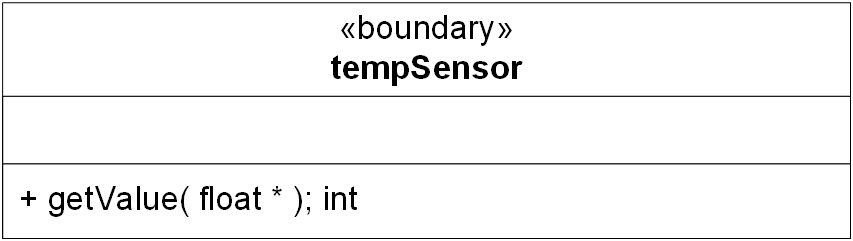
\includegraphics[scale=1.3]{filer/design/Klassediagrammer/sw_psoc_tempSensor}}
\caption{Klasse tempSensor}
\label{fig:sw_psoc_class_tempSensor}
\end{figure} 

{\centering
\textbf{tempSensor}\par
}
\textbf{Ansvar:} Håndterer kommunikationen med temperatursensor. \

\verb+void init( )+ \\
\textbf{Parametre:} Ingen. \\
\textbf{Returværdi:} Ingen. \\
\textbf{Beskrivelse:} Har ingen funktionalitet. \\

\verb+void exit( )+ \\
\textbf{Parametre:} Ingen. \\
\textbf{Returværdi:} Ingen. \\
\textbf{Beskrivelse:} Har ingen funktionalitet. \\

\verb+int getValue( float * )+ \\
\textbf{Parametre:} Pointer til at gemme temperatur i. \\
\textbf{Returværdi:} 0 ved succes ellers negativ i overenstemmelse med fejl-listen. \\
\textbf{Beskrivelse:} Sætter \verb+P_FT2+ benet lavt. Starter A/D-konvertering og omregner modtaget resultat til en temperatur i grader Celsius. \\


\begin{figure}[htbp] \centering
{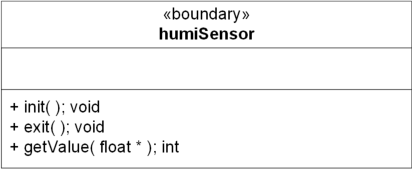
\includegraphics[scale=1.3]{filer/design/Klassediagrammer/sw_psoc_humiSensor}}
\caption{Klasse humiSensor}
\label{fig:sw_psoc_class_humiSensor}
\end{figure} 

{\centering
\textbf{humiSensor}\par
}
\textbf{Ansvar:} Håndterer kommunikationen med fugtighedssensor. \

\verb+void init( )+ \\
\textbf{Parametre:} Ingen. \\
\textbf{Returværdi:} Ingen. \\
\textbf{Beskrivelse:} Har ingen funktionalitet. \\

\verb+void exit( )+ \\
\textbf{Parametre:} Ingen. \\
\textbf{Returværdi:} Ingen. \\
\textbf{Beskrivelse:} Har ingen funktionalitet. \\

\verb+int getValue( float * )+ \\
\textbf{Parametre:} Pointer til at gemme fugtighed i. \\
\textbf{Returværdi:} 0 ved succes ellers negativ i overenstemmelse med fejl-listen. \\
\textbf{Beskrivelse:} Sætter \verb+P_FT2+ benet højt. Starter A/D-konvertering og omregner modtaget resultat til en relativ fugtighed i \%. \\

\begin{figure}[htbp] \centering
{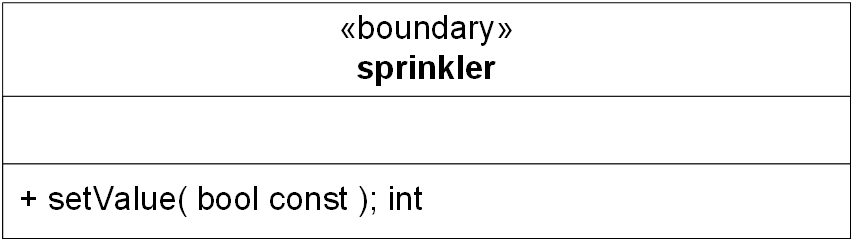
\includegraphics[scale=1.3]{filer/design/Klassediagrammer/sw_psoc_sprinkler}}
\caption{Klasse sprinkler}
\label{fig:sw_psoc_class_sprinkler}
\end{figure} 

{\centering
\textbf{sprinkler}\par
}
\textbf{Ansvar:} At aktivere og deaktivere tilkoblede sprinklere. \

\verb+void init( )+ \\
\textbf{Parametre:} Ingen. \\
\textbf{Returværdi:} Ingen. \\
\textbf{Beskrivelse:} Har ingen funktionalitet. \\

\verb+void exit( )+ \\
\textbf{Parametre:} Ingen. \\
\textbf{Returværdi:} Ingen. \\
\textbf{Beskrivelse:} Har ingen funktionalitet. \\

\verb+int setValue( unsigned char const )+ \\
\textbf{Parametre:} 1 = tænd sprinkler, 0 = sluk sprinkler. \\
\textbf{Returværdi:} 0 ved succes ellers negativ i overenstemmelse med fejl-listen. \\
\textbf{Beskrivelse:} Sætter \verb+PIN+ ud fra modtaget parameter.\\

\begin{figure}[htbp] \centering
{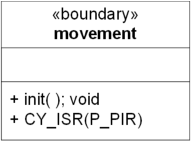
\includegraphics[scale=1.3]{filer/design/Klassediagrammer/sw_psoc_movement}}
\caption{Klasse movement}
\label{fig:sw_psoc_class_movement}
\end{figure} 

{\centering
\textbf{movement}\par
}
\textbf{Ansvar:} Registrere bevægelse fra PIR-sensor. \

\verb+void init( )+ \\
\textbf{Parametre:} Ingen. \\
\textbf{Returværdi:} Ingen. \\
\textbf{Beskrivelse:} Sætter ISR-callback funktion til P\_PIR \\

\verb+CY_ISR(P_PIR)+ \\
\textbf{Parametre:} Ingen. \\
\textbf{Returværdi:} Ingen. \\
\textbf{Beskrivelse:} Kalder \verb+movementDetect()+ i \verb+loadData+-controlleren.\\

\clearpage

% Statiske klassediagrammer
\section{Statisk klassediagram}
Efter sekvensdiagrammerne, klassediagrammet og klassebeskrivelser er designfasen så langt at der nu kan sammensættes et statisk klassediagram som viser det samlede software design. 

\subsection{Master (JC)}
%% SW klassediagram static

\begin{figure}[!htbp] \centering
{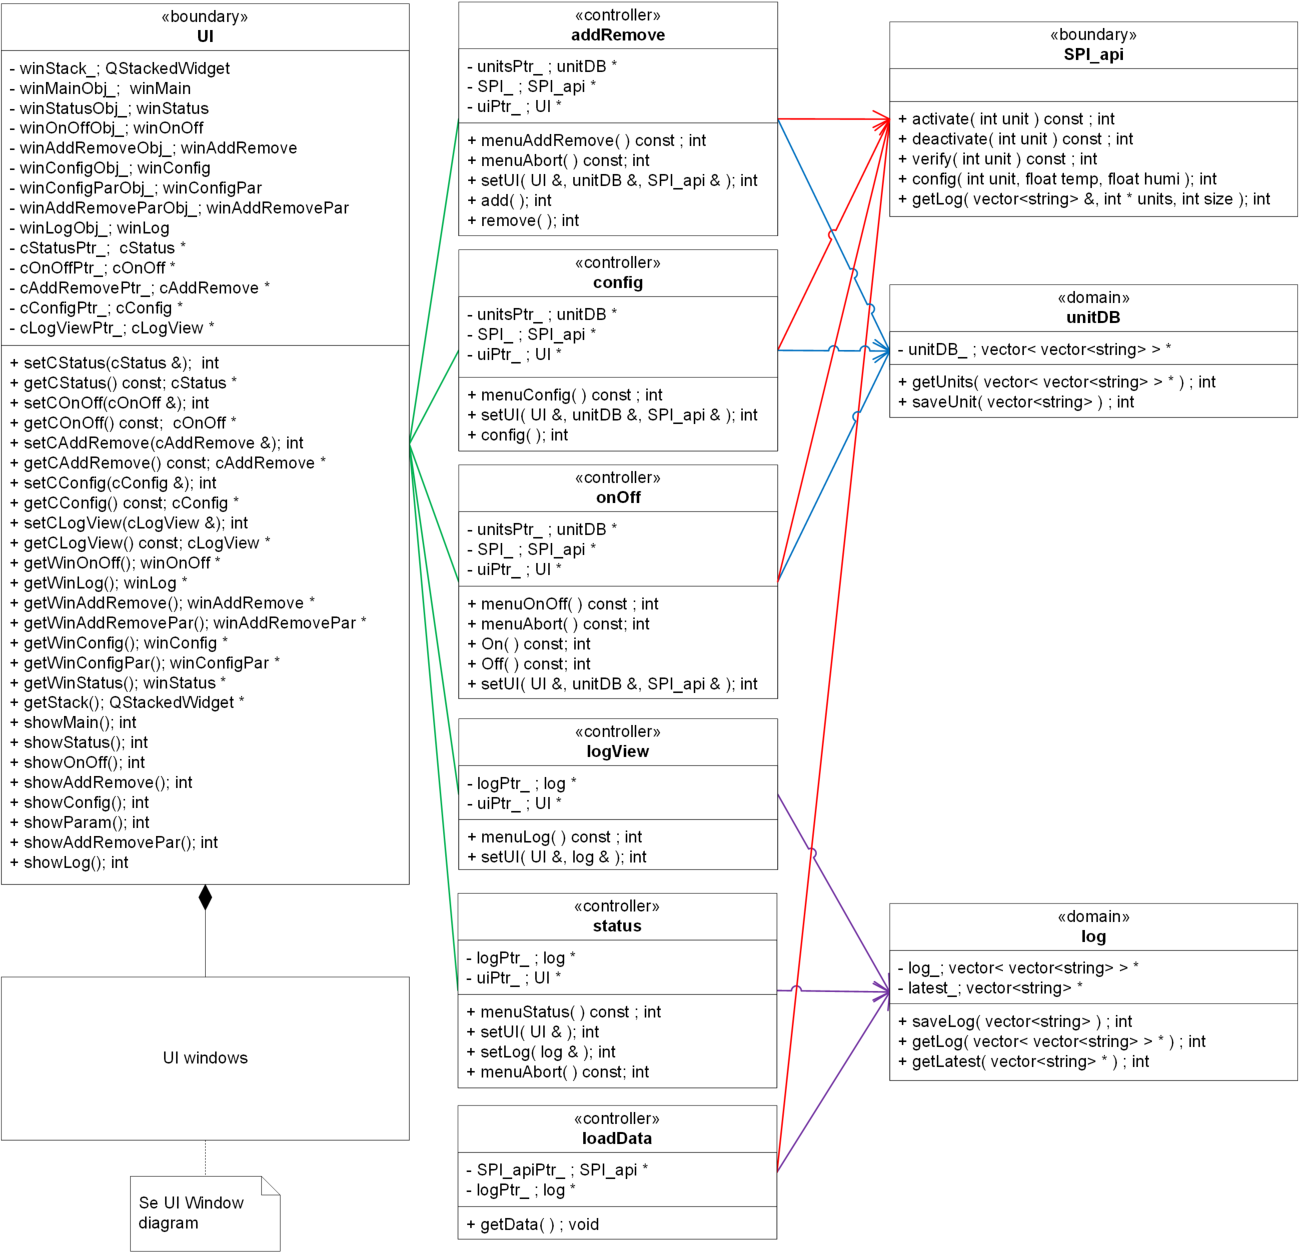
\includegraphics[scale=0.7]{filer/implementering/sw_class_devkit_static}}
\caption{Statisk klassediagram for Master (Devkit8000)}
\label{fig:class_static_dev}
\end{figure}

\begin{figure}[!htbp] \centering
{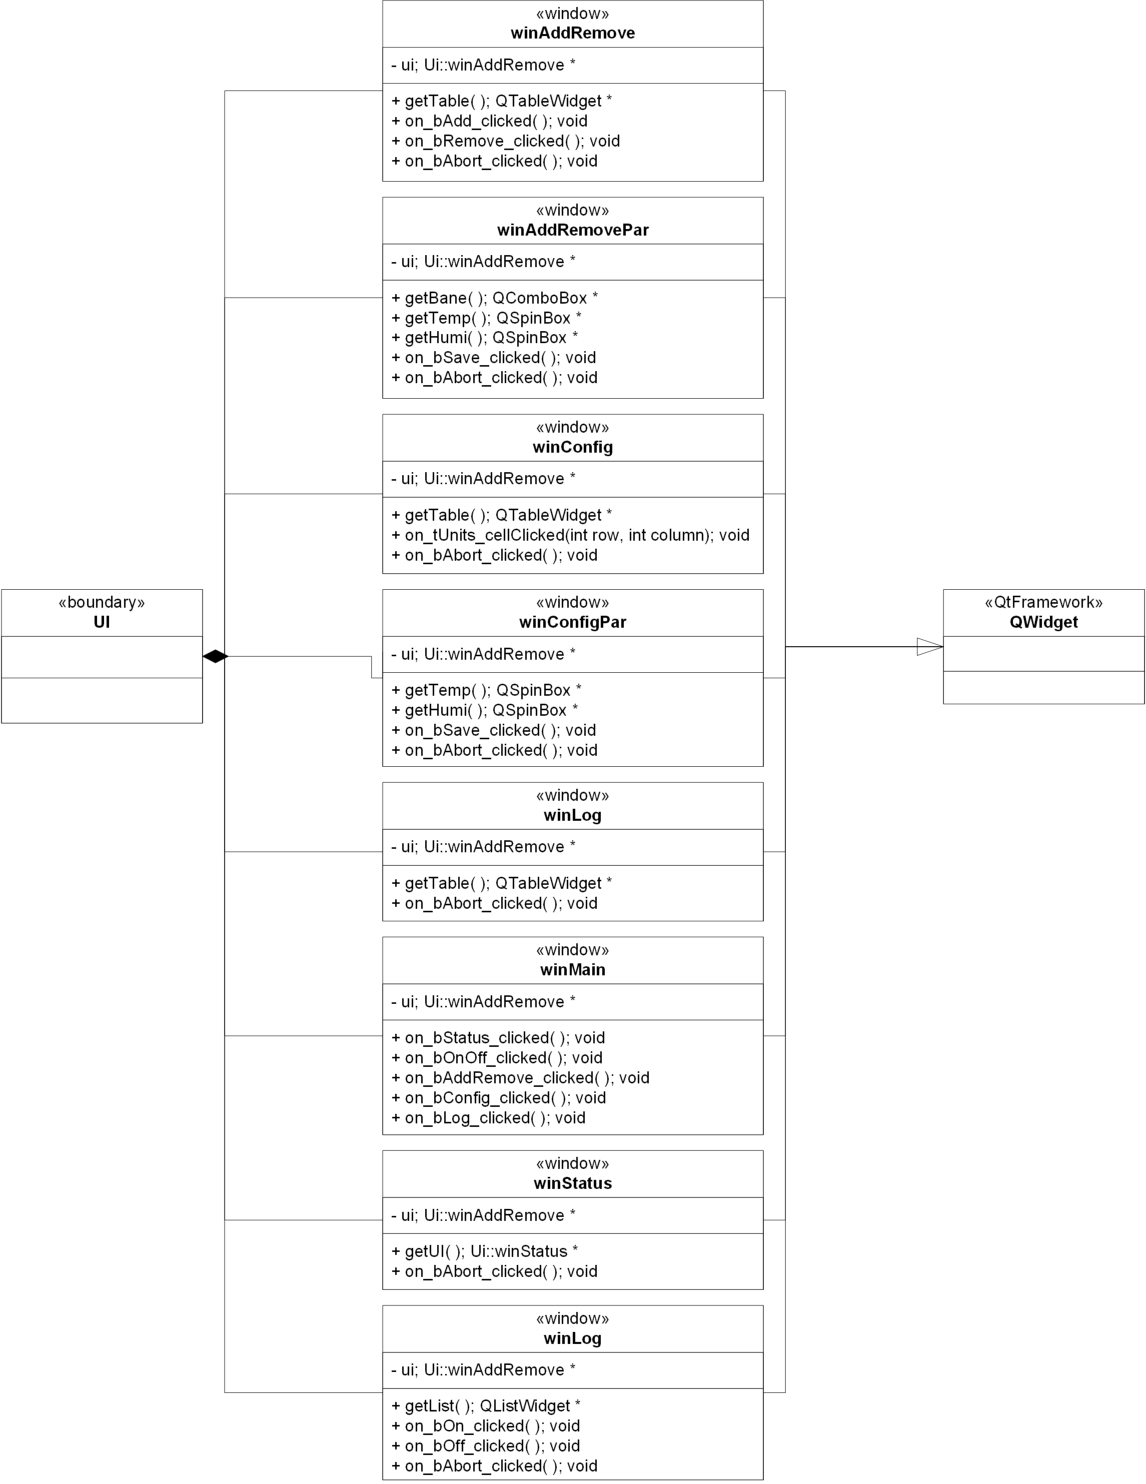
\includegraphics[scale=0.7]{filer/implementering/sw_class_devkit_windows_static}}
\caption{Statisk klassediagram for vinduer på Master (Devkit8000)}
\label{fig:class_static_dev_window}
\end{figure}


\clearpage

\subsection{Enhed (BS)}
%% SW klassediagram static

\begin{figure}[!htbp] \centering
{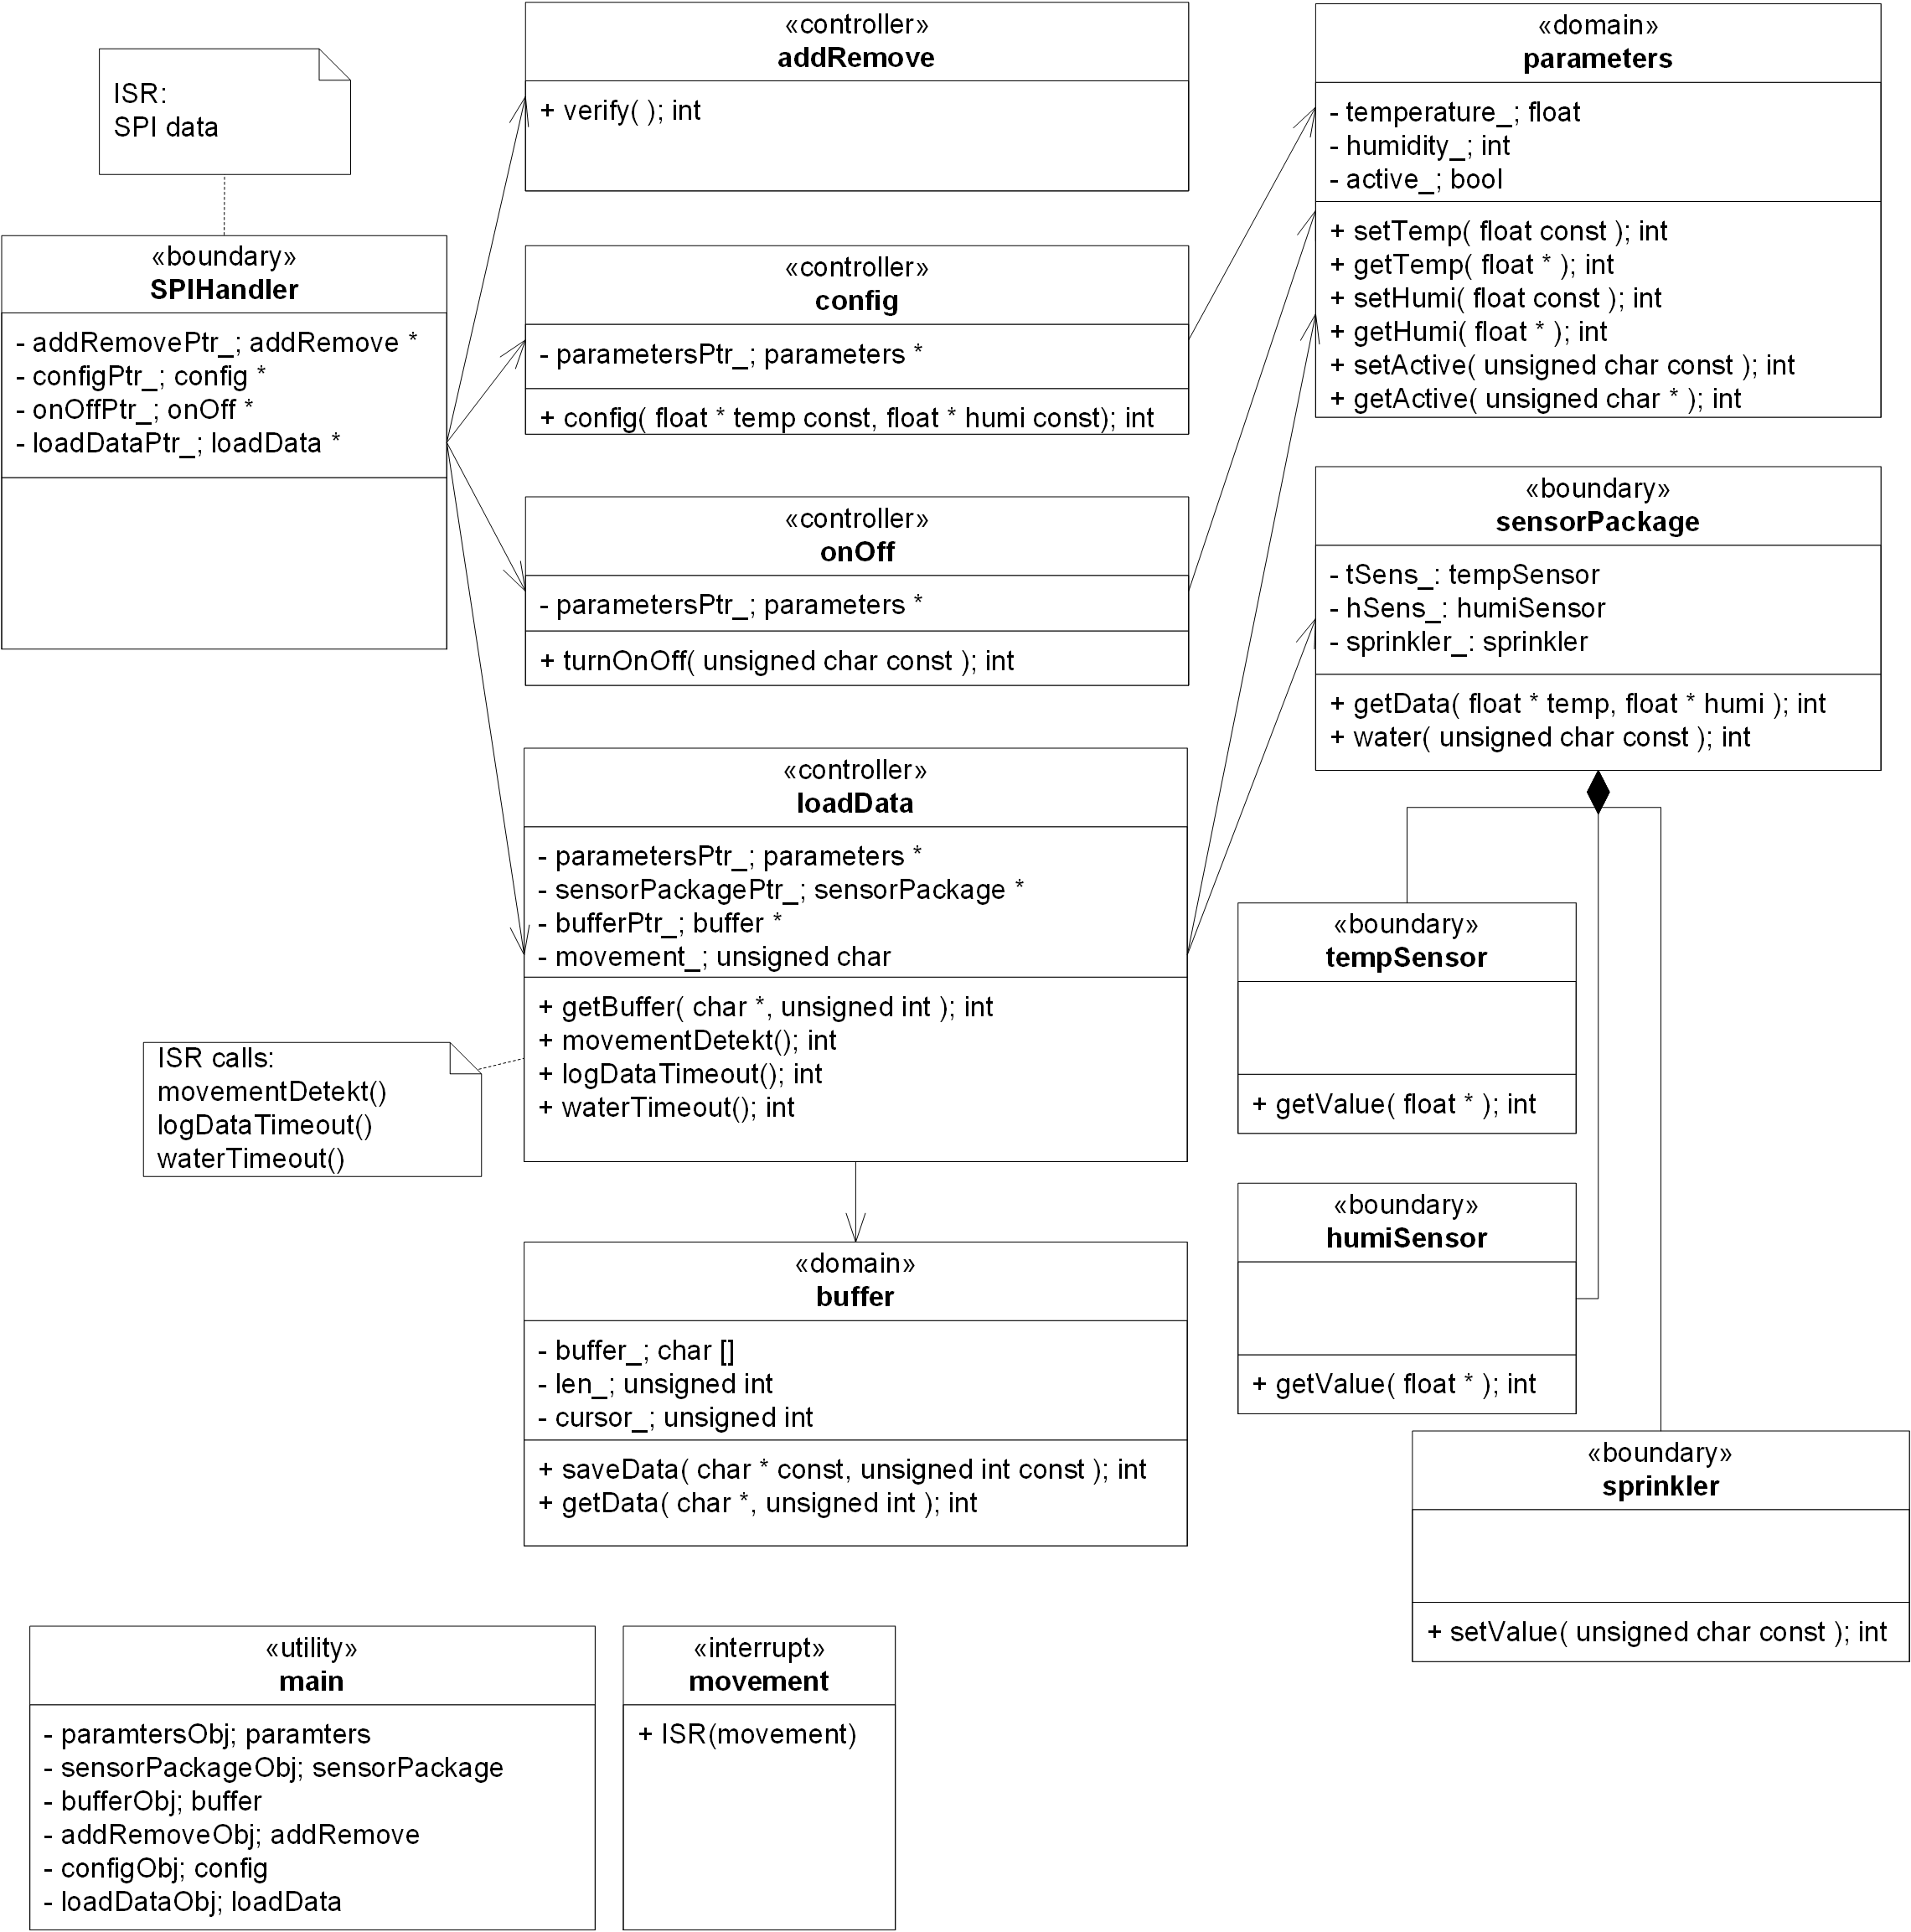
\includegraphics[scale=0.7]{filer/design/sw_class_psoc_static}}
\caption{Statisk klassediagram for Enhed (PSoC)}
\label{fig:class_psoc_static_dev}
\end{figure}




\clearpage

